\chapter{Planen des menschenzentrierten Gestaltungsprozesses}
\section{Vorgehensmodell}
Da die Anforderungen des Systems sich entwickeln und in ihrer Wichtigkeit variieren können, ist die agile Vorgehensweise in
der Konzeption des Systems erforderlich \citep[{``Agile methods are adaptive rather than predictive.''}]{TheNewMe5:online}. Da diese Umstände auch in der DIN-EN-ISO 9421-210 \citep{DINISO_2010} bereits bedacht worden sind, erleichtert das die Projektplanung maßgeblich.\\
Die Planung erfolgte durch Karten in den Kanban Boards die in Github angelegt worden sind. Somit war zu jedem Zeitpunkt klar, welche Artefakte noch erstellt oder evaluiert werden müssen. Auch die Artefakte des Entwicklungsprojekt wurden zu Beginn mit gelistet und evaluiert und dienten als Grundlage für die Anpassungen in diesem Projekt. \\

\section{Identifizieren der Personen und Organisation(en)}
\begin{wrapfigure}{r}{0.48\textwidth}
  \centering
    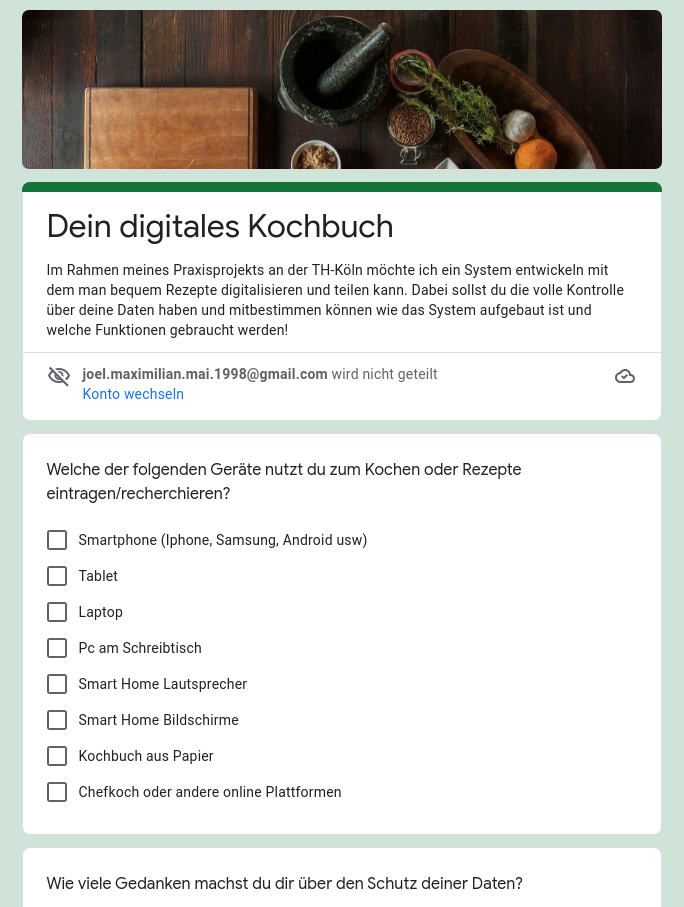
\includegraphics[width=0.25\textwidth]{images/umfrage.png}
  \centering
\caption[Google Formular (Ausschnitt)]{Google Formular (Ausschnitt)}
\label{fig:googleforms}
\end{wrapfigure}
Für die Stakeholder, die für die Priorisierung der Anforderungen interviewt worden sind, wurden aus jeder Zielgruppe zwei Personen, sofern verfügbar, in die Workshops eingeladen. 
% Mehr informationen zu den einzelnen Zielgruppen
Die Workshops bestanden aus einem Zoommeeting und einem Conceptboard-Dienst namens Miro. Vor Beginn der Meetings wurden Karten angelegt welche die Erarbeitung des User Story Mappings von Jeff Patton \citep{Patton_2014} erläutern und zur Moderation beitrugen. Im Nachgang wurden die erarbeiteten User Stories priorisiert und umformuliert. \\
 \\ \\ \\
% Anzahl der Befragten
\newpage
\section{Verfahren zur Integration der menschzentrierten Gestaltungsaktivitäten}     
Für die Evaluierung der Gestaltungslösungen und ähnlichen Artefakten wie Wireframes und LowFideltyPrototypes wurden dieselben und weitere Stakeholder über das Google Umfrage Tool {``Formulare''} interviewt um die Auswertung zu erleichtern. Dabei erhielten die Befragten vorgefertigte Antwortmöglichkeiten, aber auch Freitextfelder, um optionale individuelle Antworten zu geben. Die Auswertung der Formulare ergab Richtwerte für die Anordnungen von Elementen in den Gestaltungen. Die Ergebnisse beeinflussten auch die Entwicklung der Navigationmap und dienten als Grundlage der Evaluierung des Systems.
% Konkrete Ergebnisse einbauen

\section{Projektplanung}
Um das Projekt möglichst transparent und nachvollziehbar zu gestalten, wurden noch vor der Bearbeitung der Artefakte, Tools und Workflows ausgewählt oder erarbeitet, um den Aufwand an einzelnen Tasks und Features zu dokumentieren. Dabei wurde ein Docker Container eines Projektmanagementtools verwendet um grobe Projektphasen zu skizzieren (siehe Diagramm \ref{fig:ganttdiagramm}) und eine Exceltabelle für die automatische Errechnung des Zeitaufwands nach Markdown exportiert, um so in das \href{https://github.com/Inf166/design-concept-sharing-recipes/wiki}{Github Wiki} integriert zu werden. Dort wurden die wesentlichen Erkenntnisse und die \href{https://github.com/Inf166/design-concept-sharing-recipes/wiki/Roadmap}{Roadmap} festgehalten, die sich aus diesem Workflow ergaben.\\

\begin{figure}[h] %!=overrides latex; h=here; t=top; b=bottom; p=special page for floating objects
\centering
    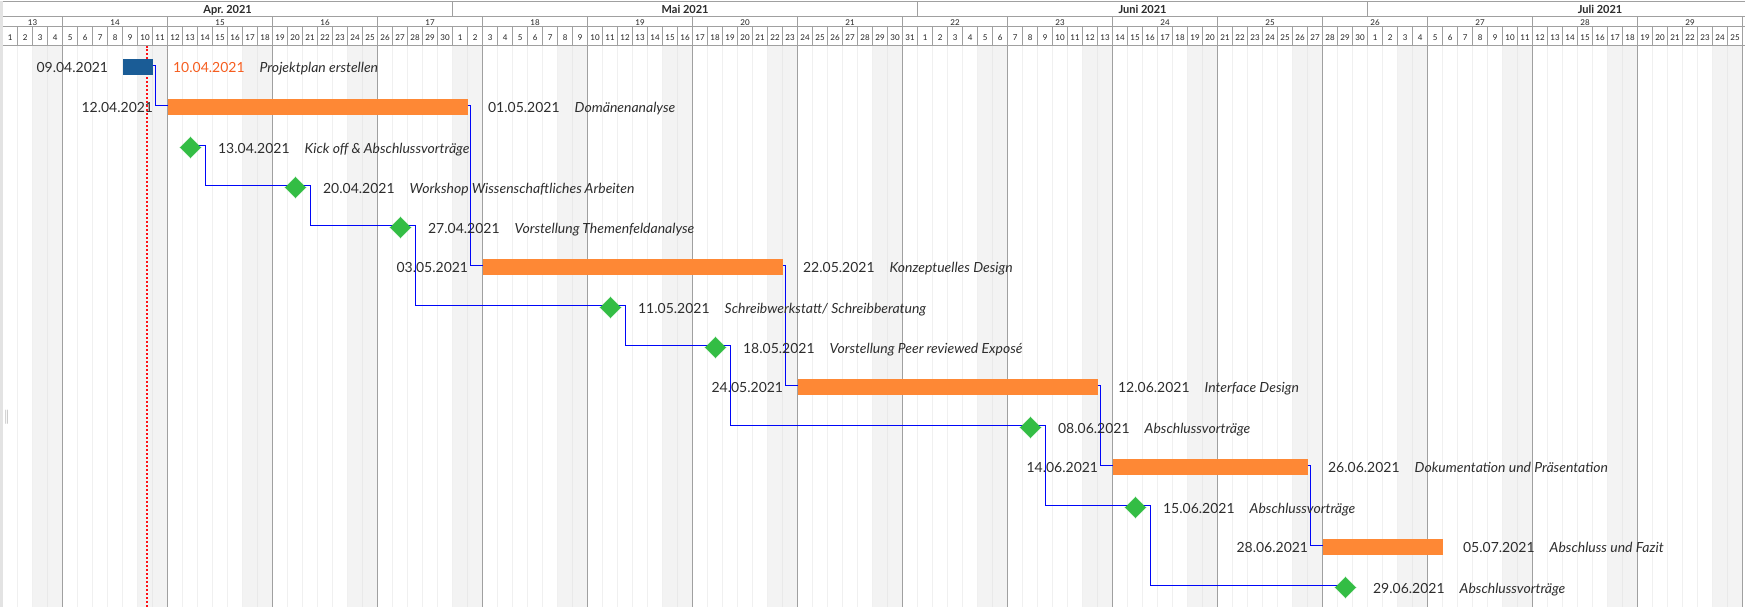
\includegraphics[width=0.8\textwidth]{images/ganttdiagramm.png}
    \caption[Ganttdiagramm]{Ganttdiagramm}
    \label{fig:ganttdiagramm}
\end{figure}
\begin{figure}[h]
\centering
    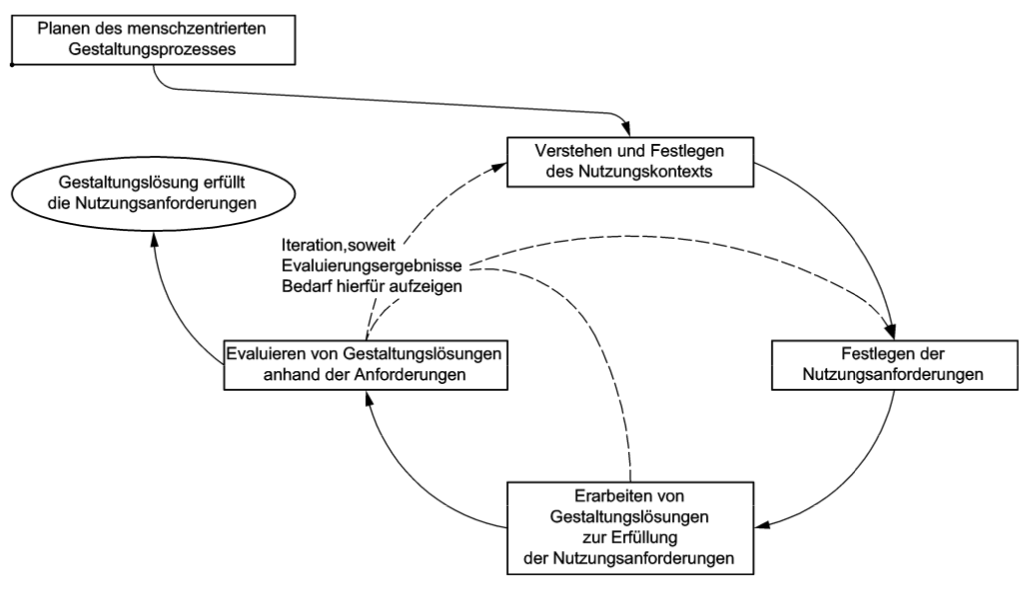
\includegraphics[width=0.5\textwidth]{images/Din-Norm-Ablaufmodell.png}
    \caption[ISO 9241-210:2010 - Bild 1]{ISO 9241-210:2010 - Bild 1}
    \label{fig:din-ablauf}
\end{figure}

\chapter{Verstehen und Festlegen des Nutzungskontexts}
Für die Anforderungsermittlung wurde das Vorgehen der DIN-EN-ISO 9241-210 \citep{DINISO_2010} (siehe Abbildung \ref{fig:din-ablauf}) gewählt. Für die Konzeption des Systems wurde hier von den bisherigen Erkenntnissen Abstand genommen und lösungsneutral das Domänenmodell überarbeitet.
% Vollständig, Notwendig, Atomar, Verfolgbar, Technisch lösungsneutral, Realisierbar, Konsistent, Eindeutig, Prüfbar, Vollständig, Konsistent, Erschwinglich, Abgegrenzt, Schnittstellenanforderung

\section{Domänenmodell}
\begin{figure}[h] %!=overrides latex; h=here; t=top; b=bottom; p=special page for floating objects
    \centering
    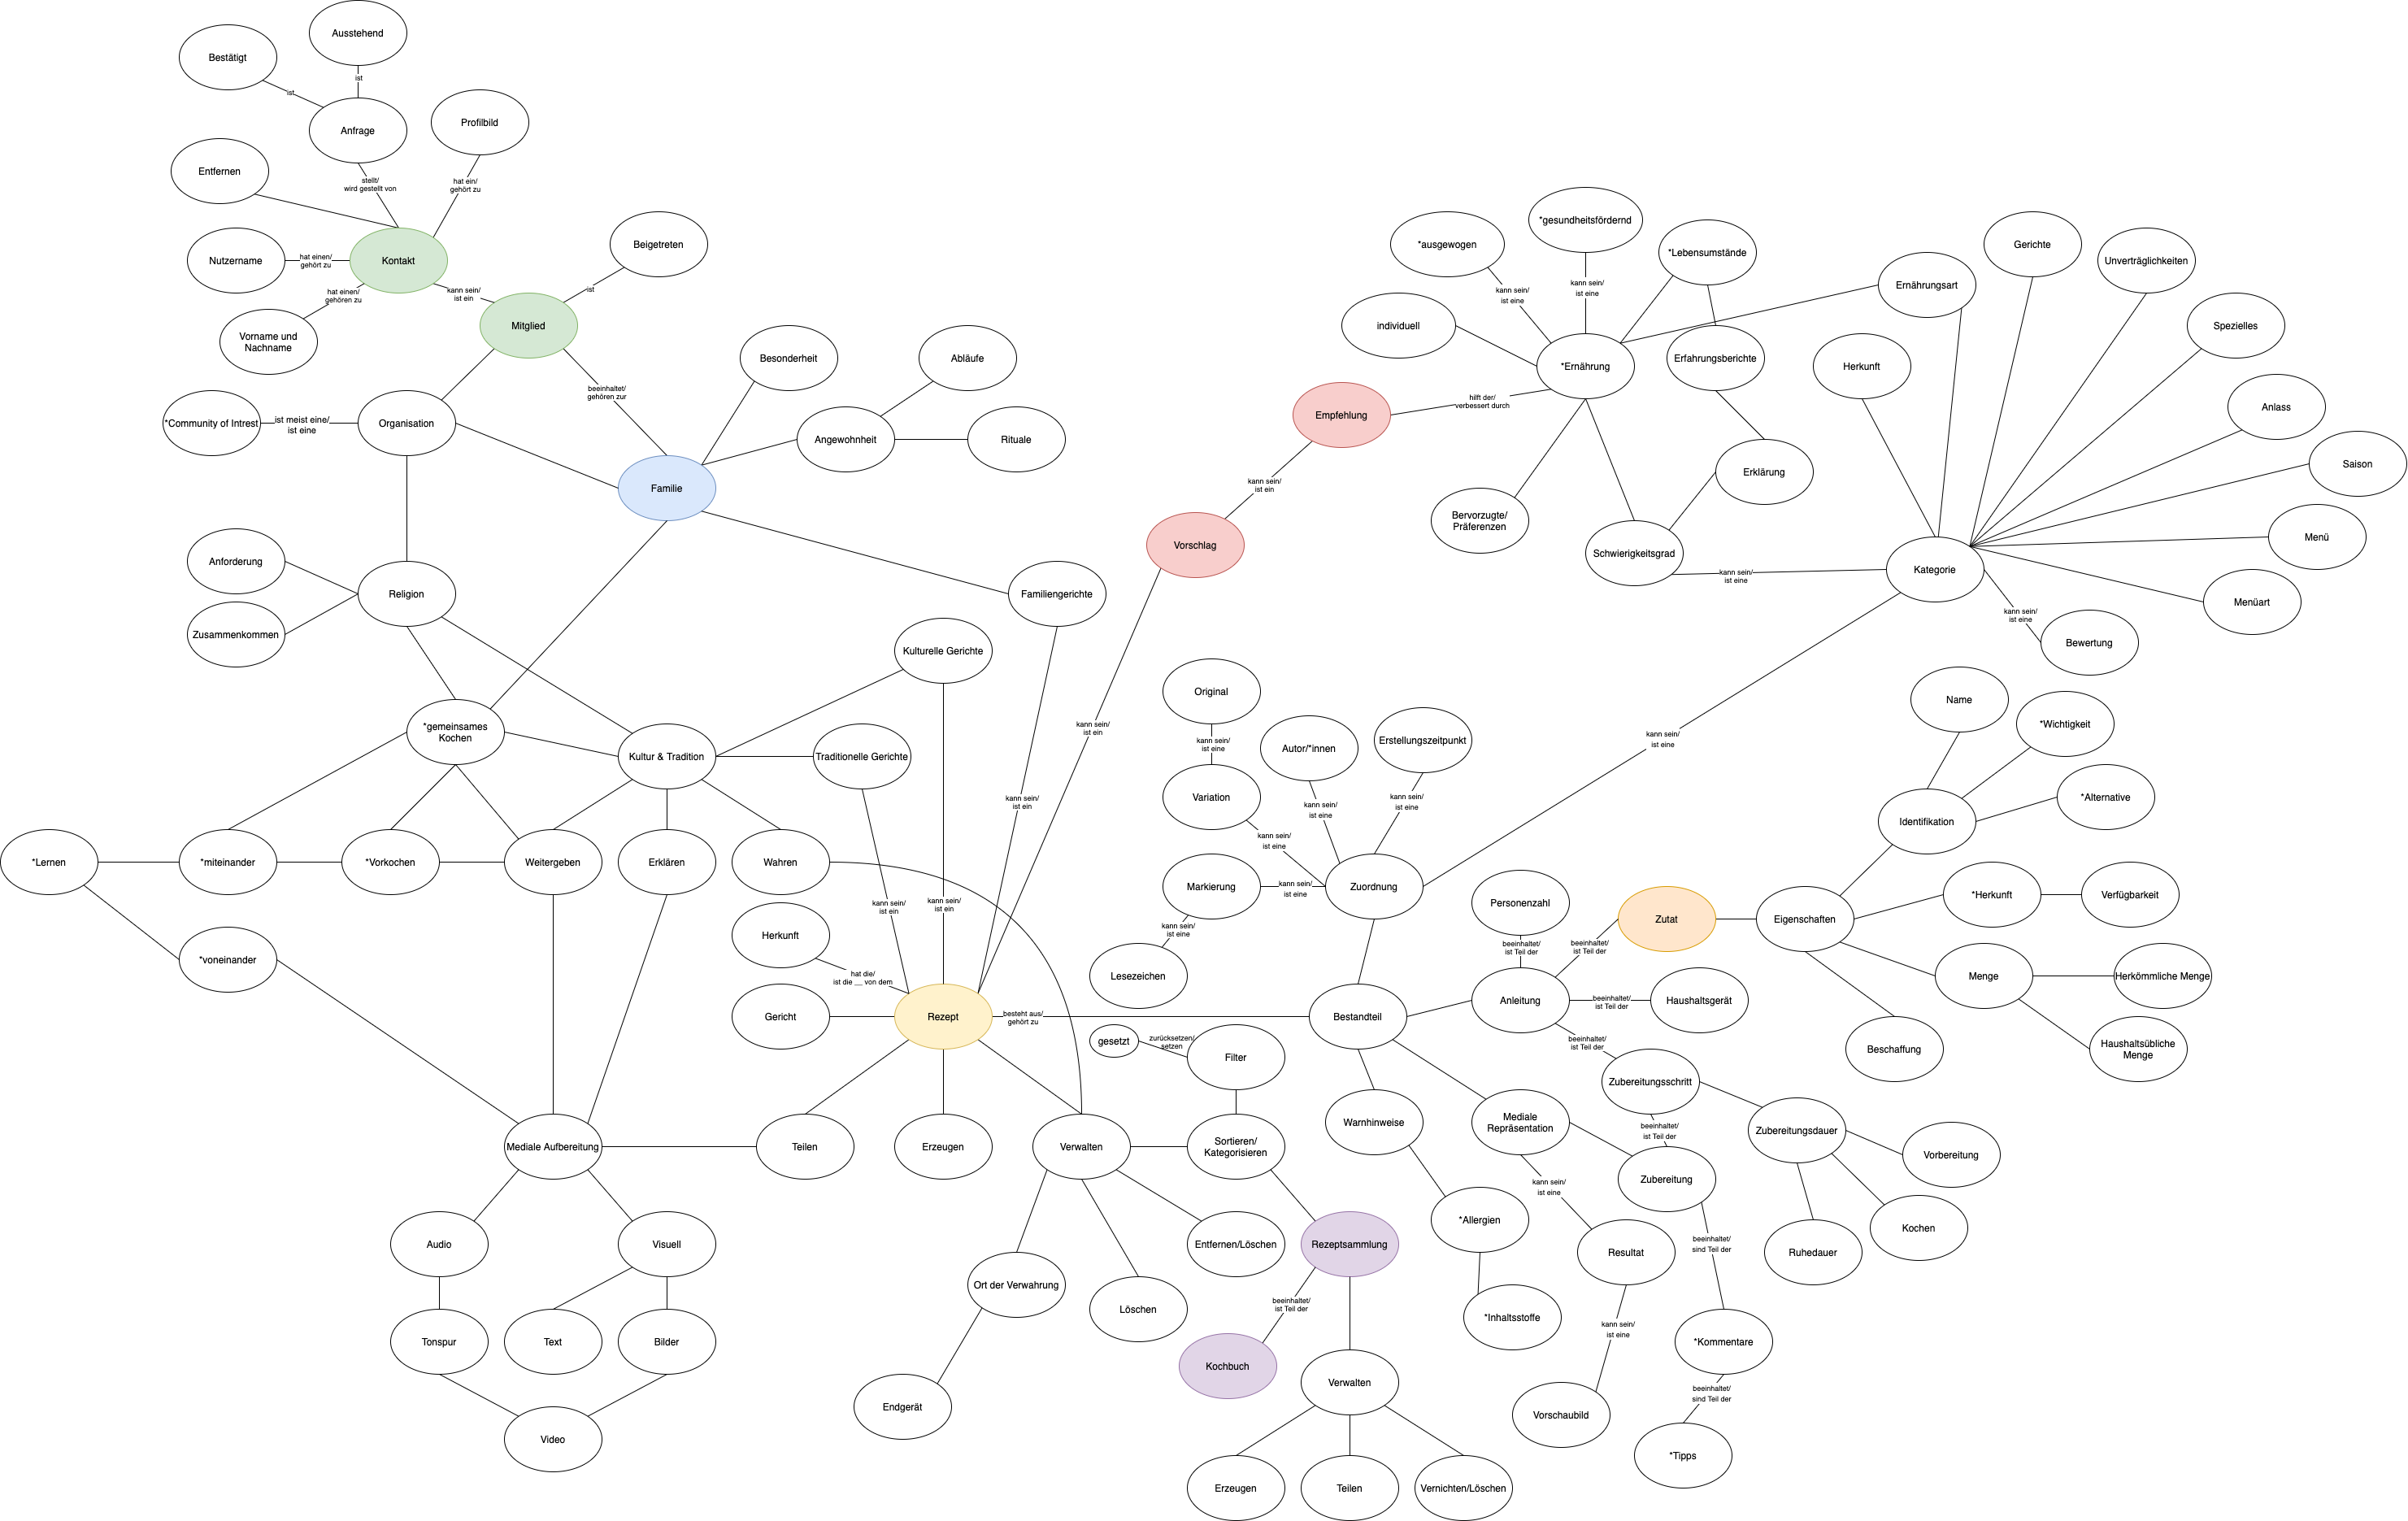
\includegraphics[width=0.8\textwidth]{images/domainmodel.png}
    \caption[Domänenmodell]{Domänenmodell}
    \label{fig:Domaenenmodell}
\end{figure}
Neben den Domänenen, wie Kochen, Rezept, Tradition, Kultur und Familie, ergeben sich hier die Erweiterung des Modells durch Religion und Zutateneigenschaften, wie zum Beispiel die Verträglichkeit, als auch die Ernährungszugehörigkeit. 
Die Differenzierung in verschiedene Domänen ergibt die Aufteilung von Zubereitung in Zubereitungsschritte und die aus den Schritten resultierende geteilte Zubereitungsdauer in Vorbereitung, Zubereitung und Anrichten. 
Diese Aufteilung ist nicht unüblich, da sie für eine mehr transparente Zubereitung sorgt und somit eine qualifiziertere Einschätzung des Rezepts ermöglichen \citep{SlowBake13:online}.\\

Haushaltsgeräte für jedes Rezept aufzulisten, ist eine Funktion, die erst mit Hilfe der Erstellung eines Domänenmodells, ermöglicht wurde. Diese Auflistung ermöglicht es den Nutzern, selbst einzuschätzen, ob ein Rezept umsetzbar ist. Auch die Unterscheidung von Vorschlag und Empfehlung ergab sich aus dem Modell, da hier unterschieden wird, ob ein Teaser den Nutzer inspirieren soll oder eine passende Alternative zu den bisher angesehenen Rezepte ist.\\

\chapter{Festlegen der Nutzeranforderungen}
\label{sec:userstories}
\begin{figure}[h] %!=overrides latex; h=here; t=top; b=bottom; p=special page for floating objects
    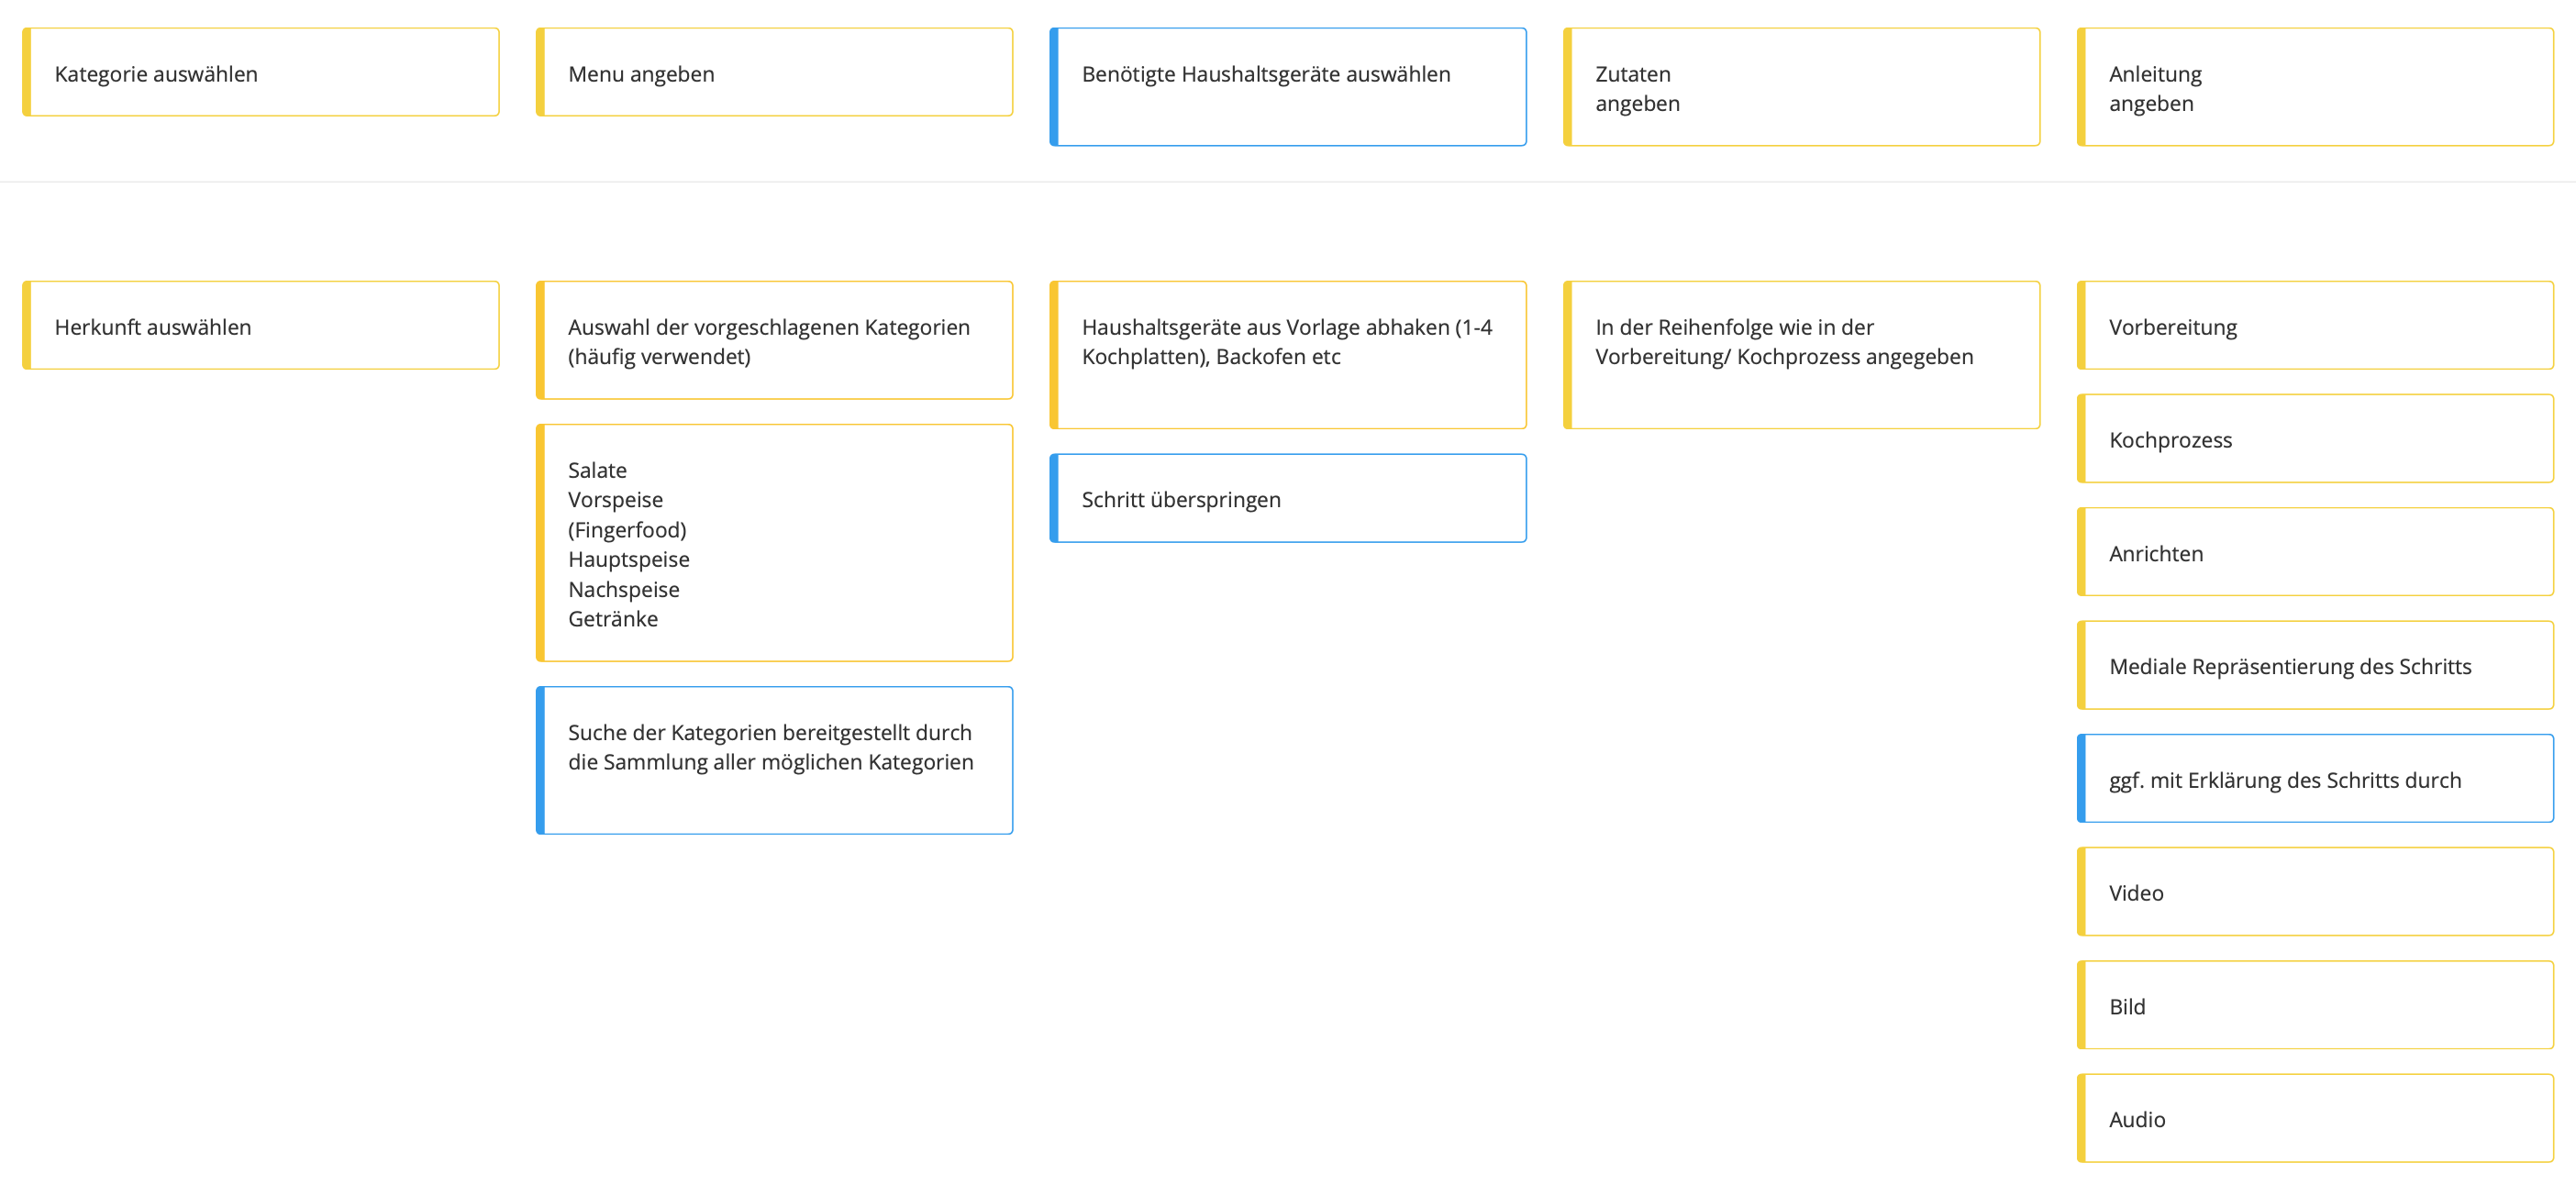
\includegraphics[width=1\textwidth]{images/userstories.png}
    \caption[User Stories (Ausschnitt)]{User Stories (Ausschnitt)}
    \label{fig:userstories}
\end{figure}
Um später bestimmen zu können, ob die Anforderungen erfüllt worden sind, wurde mit den potenziellen Nutzern ein Workshop zur Erarbeitung der User Stories und die Priorisierung für das Minimum Viable Product (MVP)\citep{Patton_2014} abgehalten. Dabei ergaben die Ergebnisse die geringe Wichtigkeit und Bedeutung von Datenschutz im Sinne des Ablageortes der Daten der jeweiligen Nutzer. Für die Nutzer ist eine verschlüsselte Datenbank unabhängig von großen Konzernen wie Google und Amazon ausreichend.\\ 

Desweiteren wurde eine gemeinsame Kundensprache konzipiert, wie zum Beispiel die Titel der einzelnen Schwierigkeitsgrade (Einfach, Normal, Anspruchsvoll). Zusätzlich zu aufgeteilten Angaben der Zubereitungsdauer (Vorbereitung, Zubereitung, Anrichten), soll die Backzeit, Temperatur als auch die Backofen-Einstellung angegeben werden können. Durch vordefinierte Kategorien soll die Zuordnung und das Wiederfinden erleichtert werden. Haushaltsgeräte anzugeben, soll übersprungen werden können. Die Angabe von Zutaten soll mit einem Hinweis erweitert werden, die Zutaten in der Reihenfolge anzugeben, wie sie auch in der Zubereitung verwendet werden, um das Nachkochen zu erleichtern. Rezepte sollen als {``Privat''} markiert werden können und dementsprechend nicht von anderen eingesehen werden können.\\ 

Weniger wichtige Punkte sind die automatische Generierung von Kalorien und Inhaltsstoffen der Zutaten. Besonders wichtig und von allen Teilnehmern gewünscht, ist die Funktion, dass der Bildschirm sich während des Kochens nicht abschaltet, um die Lesbarkeit der Zubereitungsschritte zu gewährleisten. Optional soll die Darstellung der einzelnen Schritte hier von dem konzipierten Auflisten abweichen und besonderen groß dargestellt werden, um die Lesbarkeit aus der Ferne zu garantieren. Auch die Sprachsteuerung wurde diskutiert, um bei schmutzigen Händen trotzdem zwischen den einzelnen Schritten navigieren zu können.\\ 

Im Nachgang an den Kochprozess oder bei dem Anlegen eines Rezepts können von Nutzern persönliche Anekdoten, Tipps und Tricks oder einfache Kommentare verfasst werden. Um die Veränderungen in Familienrezepten über mehrere Generation besser nachvollziehen zu können, werden sowohl das Originalrezept, als auch der Vorgänger des aktuell betrachteten Rezepts dem Nutzer präsentiert.
 % Zuweisen von Ressourcen, sowohl um frühzeitige Rückmeldungen zur Verbesserung des Produkts zu erhalten als auch, in einer späteren Phase, um zu bestimmen, ob die Anforderungen erfüllt wurden;
% --> Use–Case–Modellierung

\section{Content und Navigation Map}
\begin{figure}[h] %!=overrides latex; h=here; t=top; b=bottom; p=special page for floating objects
    \centering
    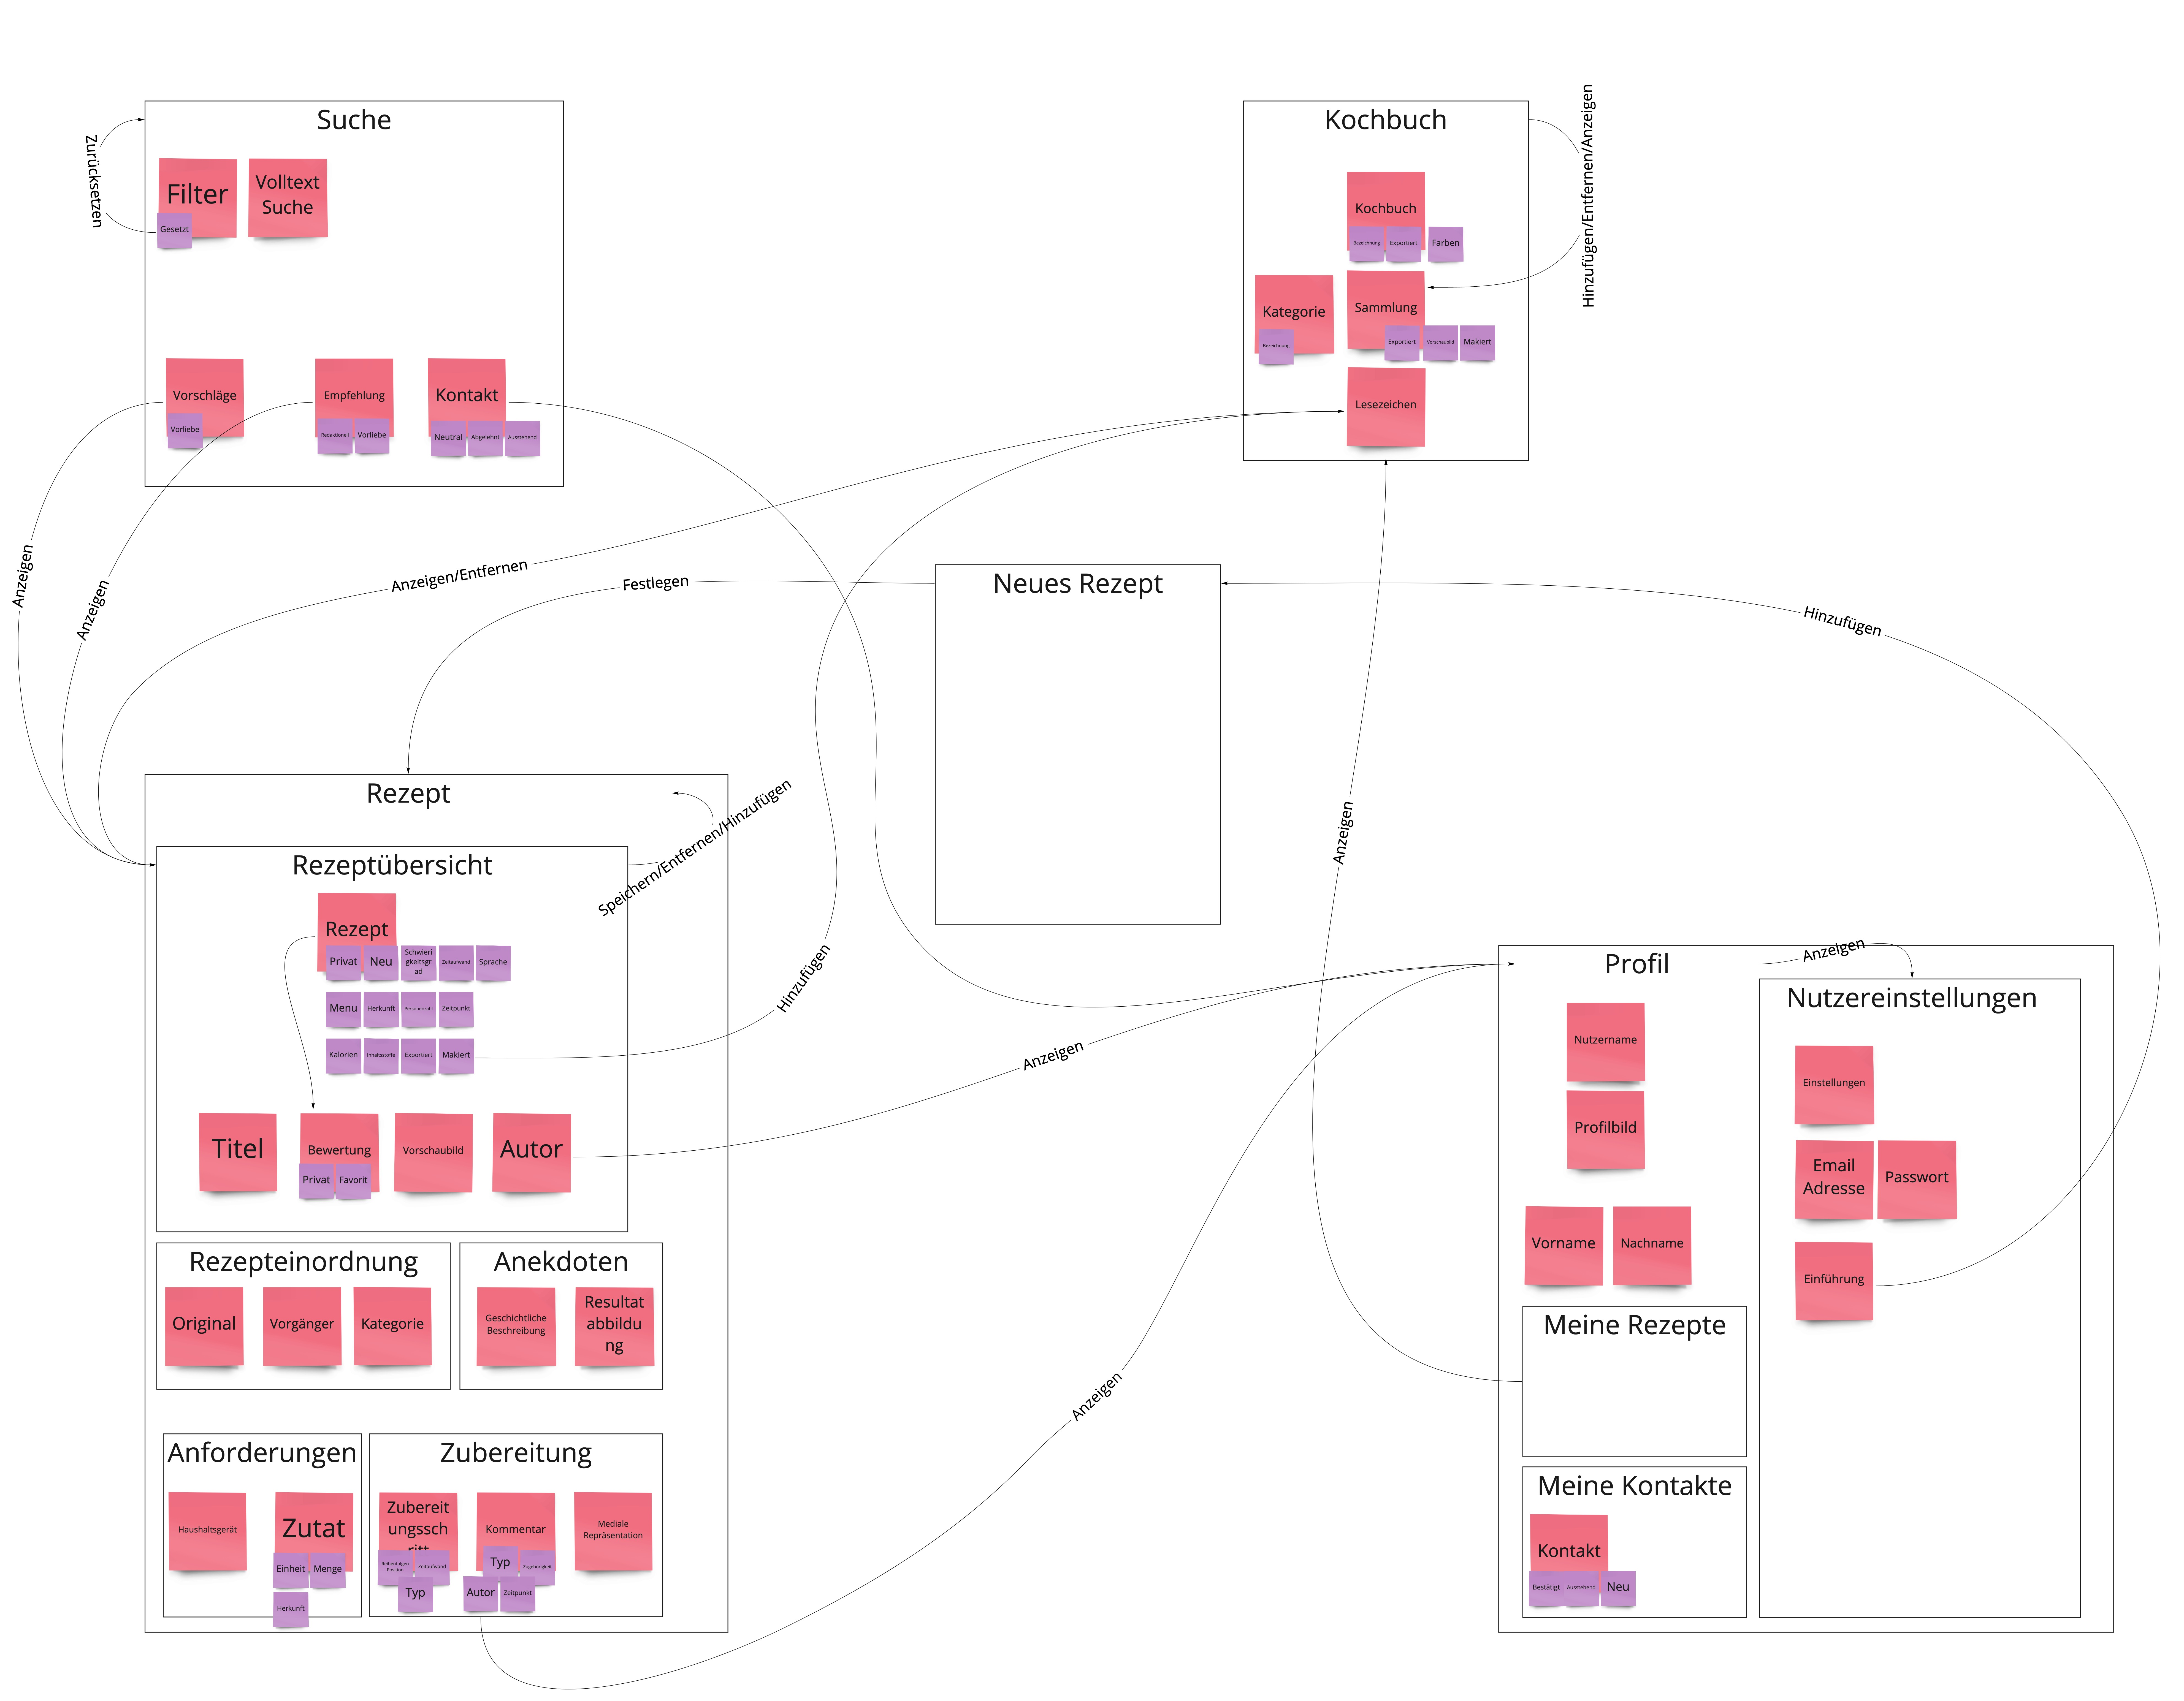
\includegraphics[width=0.9\textwidth]{images/navigationmap.jpg}
    \caption[Content Map erweitert zur Navigation Map]{Content Map erweitert zur Navigation Map}
    \label{fig:navigationmap}
\end{figure}
Um die Navigation des Systems so selbsterklärend wie möglich zu gestalten, wurden die User Stories nach der KJ method \cite[Kavakita Jiro]{KJmethod_1997} in einem Affinitäts-Diagramm nach Content Objekten gefiltert und die Duplikate in den verschiedenen Clustern reduziert. Anschließend wurden zwischen den Objekten durch die erhaltenen Verben Verbindungen gezogen, die später die Navigationswege darstellen sollen. Zusätzliche Objekte oder Zustände wurden in lila Karten dargestellt und zu den jeweiligen Objekten angeheftet.\\

Neben klar geclusterten Gruppen wie Kochbuch, Suche und Neues Rezept, bewies die Clusterung des Rezepts sich als Herausforderung. Hier war die Einteilung in Untergruppen besonders komplex. Das Cluster Rezeptübersicht soll wesentliche Informationen eines Rezepts beinhalten, jedoch nicht die einzelnen Schritte eines Rezepts, da diese die Übersicht überladen würden. Die Rezepteinordnung hat im Wesentlichen nichts mit dem eigentlichen Rezept zu tun, daher wird auch sie getrennt von dem Rezept und in ein eigenes Cluster verschoben. Für die Anekdoten gilt selbiges. Die Anforderungen beinhalten die Zutaten und Haushaltsgeräte und sind für die Zubereitung zwar wesentliche Bestandteile, jedoch keine Zubereitungsschritte.\\ 

Daraus ergibt sich das letzte Cluster: Zubereitung. Hierzu gehört der Zubereitungsschritt, dessen Position in der Zubereitungsreihenfolge, der Zeitaufwand und die Bezeichung/Typ des Schritts. Zu diesem Zeitpunkt war geplant, dass für jeden Schritt einzelne mediale Repräsentationen, aber auch das Kommentare und die dazu gehörigen Typen von Kommentaren zu jedem Schritt hinzugefügt werden können. Dieser Gedanke wurde jedoch wieder verworfen - einerseits durch die Reduzierung der Funktionen des MVPs, aber auch durch Evaluierung anhand der potentiellen Nutzergruppe.\\ 

Das Profil ist in die Übersichtsobjekte eines Profils unterteilt und erweitert durch die eigenen, besonders gekennzeichneten Rezepte und die Kontakte, die dieses Profil hält. Aus der Recherche hat sich ergeben, dass die meisten sozialen Dienste die Einstellungen zu dem eigenen Konto oder der Applikation meistens in der Profilansicht anordnen. Daher ist es naheliegend, um die Lernbarkeit des Systems zu gewährleisten, auch hier die Einstellungen zum Profil zuzuordnen. \\

% Erläutern, warum einzelne Empfehlungen nicht anwendbar sind;

\chapter{Erarbeitung von Gestaltungslösungen zur Erfüllung der Nutzungsanforderungen}
Anhand der Content Map und der dort erarbeiteten Cluster sollen nun im Zusammenspiel mit der Navigation Map Gestaltungslösungen erarbeitet werden, die die Nutzeranforderung erfüllen. Dabei wurde in jedem Schritt die Evaluierung der bisherigen Lösung durchgeführt und alternative Lösungen präsentiert. Anhand der Auswahl der Gestaltungslösungen konnten die Nutzergruppen eine zufriedenstellende Lösung auswählen.
% Kurz die Roadmap erklären und das einbeziehen/den Einbezug der Nutzergruppe

\section{Wireframes}
\begin{wrapfigure}{r}{0.4\textwidth}
  \centering
    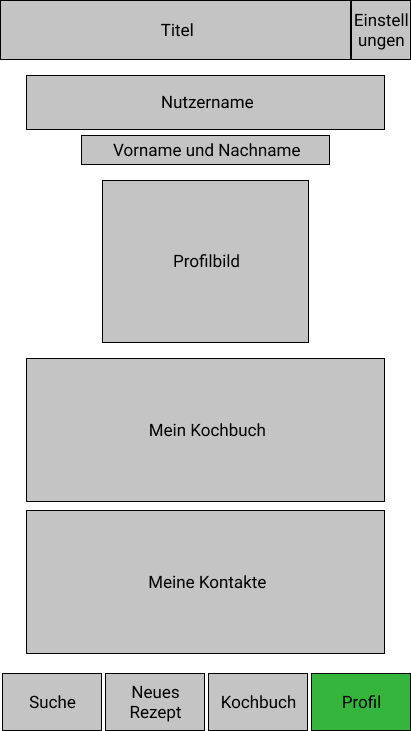
\includegraphics[width=0.25\textwidth]{images/wf-profil.jpg}
  \centering
\caption[Wireframe - Profil]{Wireframe - Profil}
\label{fig:wfprofil}
\end{wrapfigure}
Für die Gewährleistung der Konformität der Benutzererwartungen wurden die Cluster aus der Navigation Map möglichst nach Priorität für die Nutzer auf den verschiedenen Endgeräten angeordnet. Auf der Abbildung \ref{fig:wfprofil} erkennt man deutlich die Cluster aus der Abbildung \ref{fig:navigationmap} wieder. Im oberen Bereich, welcher auf den ersten Blick am besten gelesen werden kann, angeordnet sind die Informationen, die für das Cluster am wichtigsten waren.\\ 
Die Navigation, welche die wahrscheinlich häufigste Interaktion zu erwarten hat, befindet sich, für den Nutzer am leichtesten erreichbar, an dem unteren Bildschirmrand. Ganz oben am Bildschirmrand, mit der wahrscheinlich wenigsten Interaktion im Alltagsgebrauch, befindet sich die Titelleiste, ergänzt um die Einstellungen. \\ Dasselbe Verfahren wurde für die übrigen Wireframes verwendet und von den Nutzern als zufriedenstellend bewertet. \\
% Konformität mit Benutzererwartungen

\section{Styleguide}
\label{subsec:styleguide}
Um an die Gestaltung traditioneller Kochbücher anzulehnen, wurden noch vor der Gestaltung einzelner Screens, die Farbpalette und Schriftarten ausgewählt. Für die Farbpalette wurden verschiedene Fotografien von Gerichten auf ihre Farben analysiert und auf typische Farbpaletten aus der Web Entwicklung, wie zum Beispiel Bootstrap, abgebildet. Das ergab die primären Farben des Systems \citep{colortheme_2019}.  \\
\begin{figure}[h] %!=overrides latex; h=here; t=top; b=bottom; p=special page for floating objects
    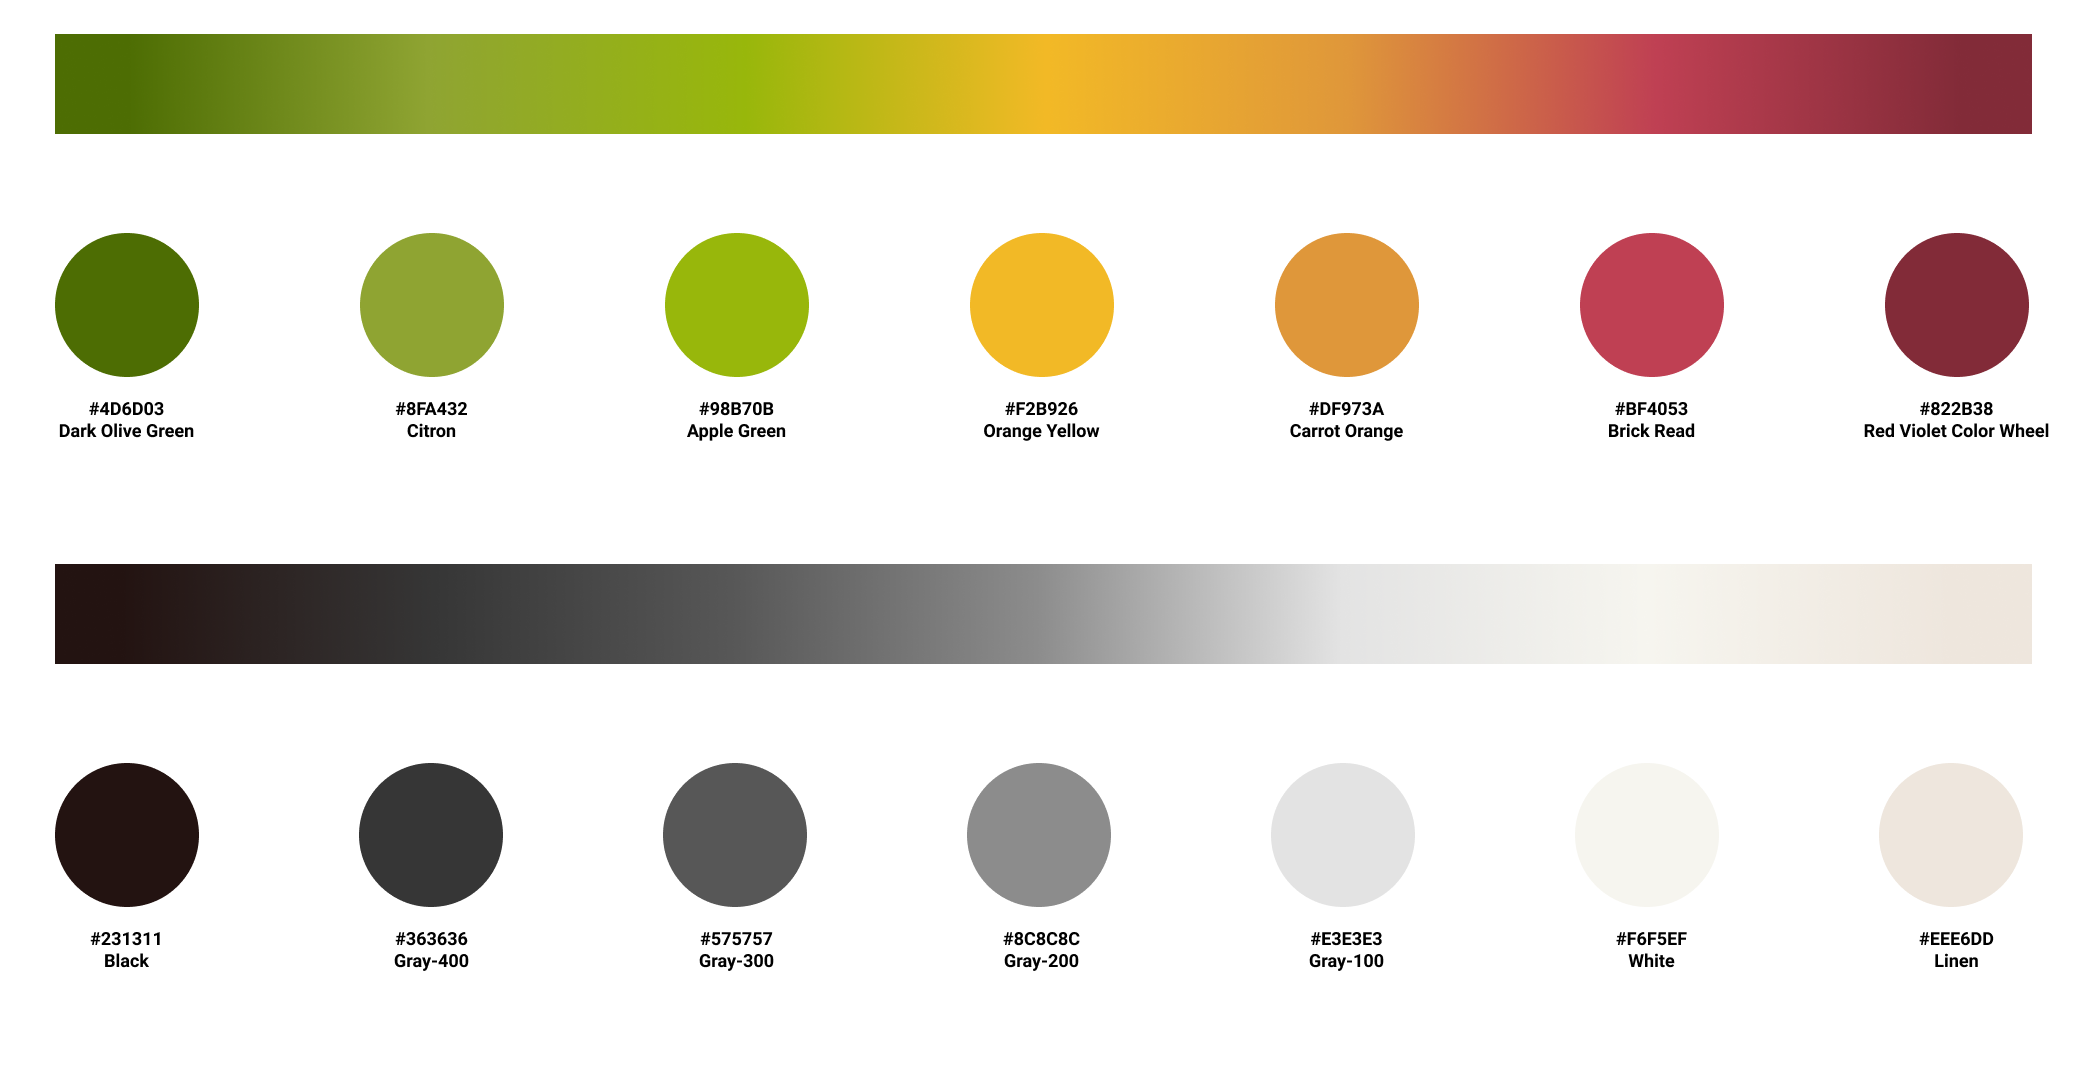
\includegraphics[width=1\textwidth]{images/colorscheme.png}
    \caption[Farbschema für den Styleguide]{Farbschema für den Styleguide}
    \label{fig:styleguide-colorscheme}
\end{figure}
\\
Für die Schriftarten wurden freie Schriftarten auf ihre charakteristischen Eigenschaften analysiert und auf ein Demorezept angewendet, um für verschiedene Aufgaben auch die korrekte Schriftart zu wählen. Nutzern wurden diese verschiedenen Lösungen präsentiert und dann evaluiert. Ein wichtiger Einwand ist hier die Verfügbarkeit dieser Schriften, da sie mit jeder Nutzung auch heruntergeladen werden müssen. Letztendlich wurden verschiedene Schriftfamilien für das System ausgewählt. \\
Die ausgewählten Schriften lauten: \\
\begin{minipage}{.7\textwidth}
    \begin{tabular}{ l l l }
        \textbf{Schriftfamilie} & \textbf{Schriftart} & \textbf{Schriftgröße} \\ 
        Roboto & Regular & 33px \\  
        Roboto & Regular & 27px \\
        Roboto & Regular & 23px \\
        Roboto & Bold & 19px \\
        Roboto & Bold & 16px \\
        Roboto & Regular & 16px \\
        Patrick Hand SC & Regular & 16px \\
        Roboto Slab & Bold & 11px \\
        Roboto & Bold & 11px \\
    \end{tabular}
\end{minipage}
\begin{minipage}{.3\textwidth}
    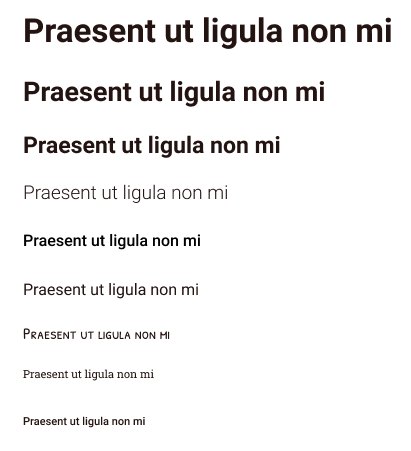
\includegraphics[width=1\textwidth]{images/typographie.png}
    \label{fig:styleguide-typographie}
\end{minipage}

Um die Erstellung der Gestaltungslösungen zu erleichtern, wurde nach dem \href{https://atomicdesign.bradfrost.com/chapter-2/}{Atomic Design} ein Styleguide erarbeitet, der die verschiedenen Gestaltungselemente eines Systems in verschiedene Gruppen aufteilt.
% hier die Aufteilung ergänzen
Die Aufteilung soll gerade die Erarbeitung mit Tools wie \href{https://www.figma.com/}{Figma} erleichtern. So braucht man nur die Original Komponente zu verändern/anzupassen und diese Änderungen werden automatisch im gesamten Design übernommen. Folglich können neue Anforderungen effizient umgesetzt werden. \\

Da die Interaktionsflächen Aufgaben angemessen und selbstbeschreibend sein sollen, wurden etablierte Muster wie Karten in Übersichten und Karussellen für Galerien für diesen Use Case angepasst und in das Design integriert. Somit sollten bekannte Strukturen wie Ordner in Ordnern erleichtert visualisiert werden und die Benutzbarkeit stärken. Als weitere Orientierungshilfe sind hier noch die \href{https://developer.apple.com/design/human-interface-guidelines/}{Human Design Guidelines} \citep{HumanInt45:online} und das \href{https://material.io/design}{Material Design} \citep{DesignMa23:online} zu nennen, da diese die Grundlage bilden, um ein System so zu gestalten, dass sowohl für IOS, als auch Android Nutzer, eine gewisse Vertrautheit besteht \citep{Mitrovic2016ARO}.
\clearpage

\section{Mock Ups}
\begin{wrapfigure}{r}{0.38\textwidth}
    \centering
        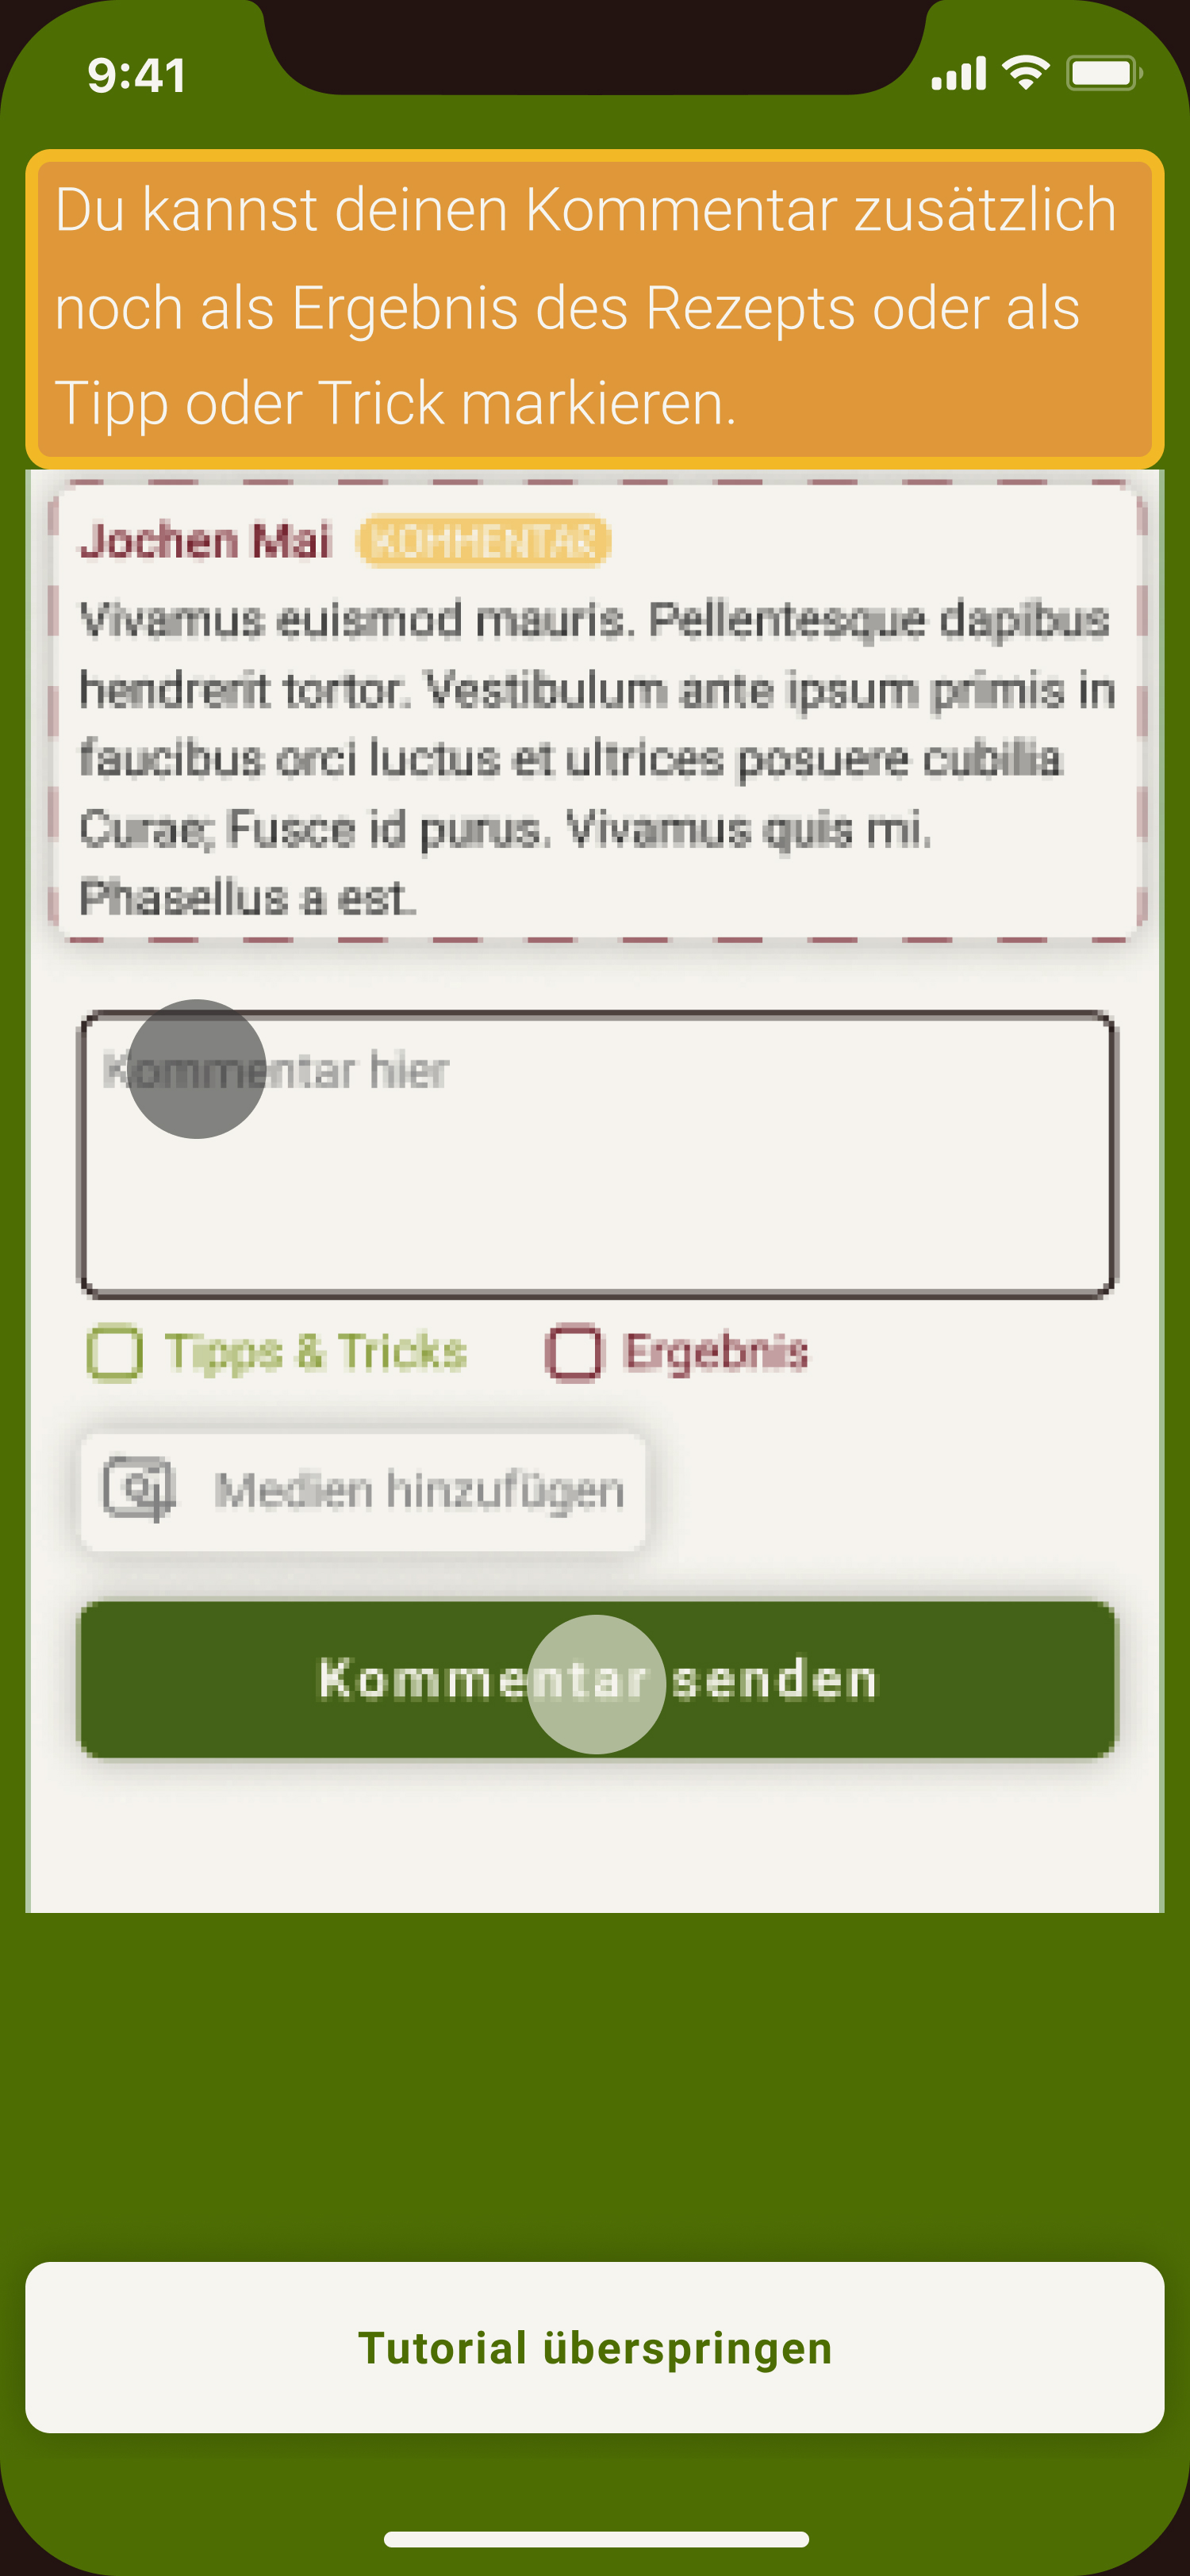
\includegraphics[width=0.14\textwidth]{images/introduction.jpg}
    \caption[Mock Up - Einführung]{Mock Up - Einführung}
\label{fig:mockup-introduction}
    \center
        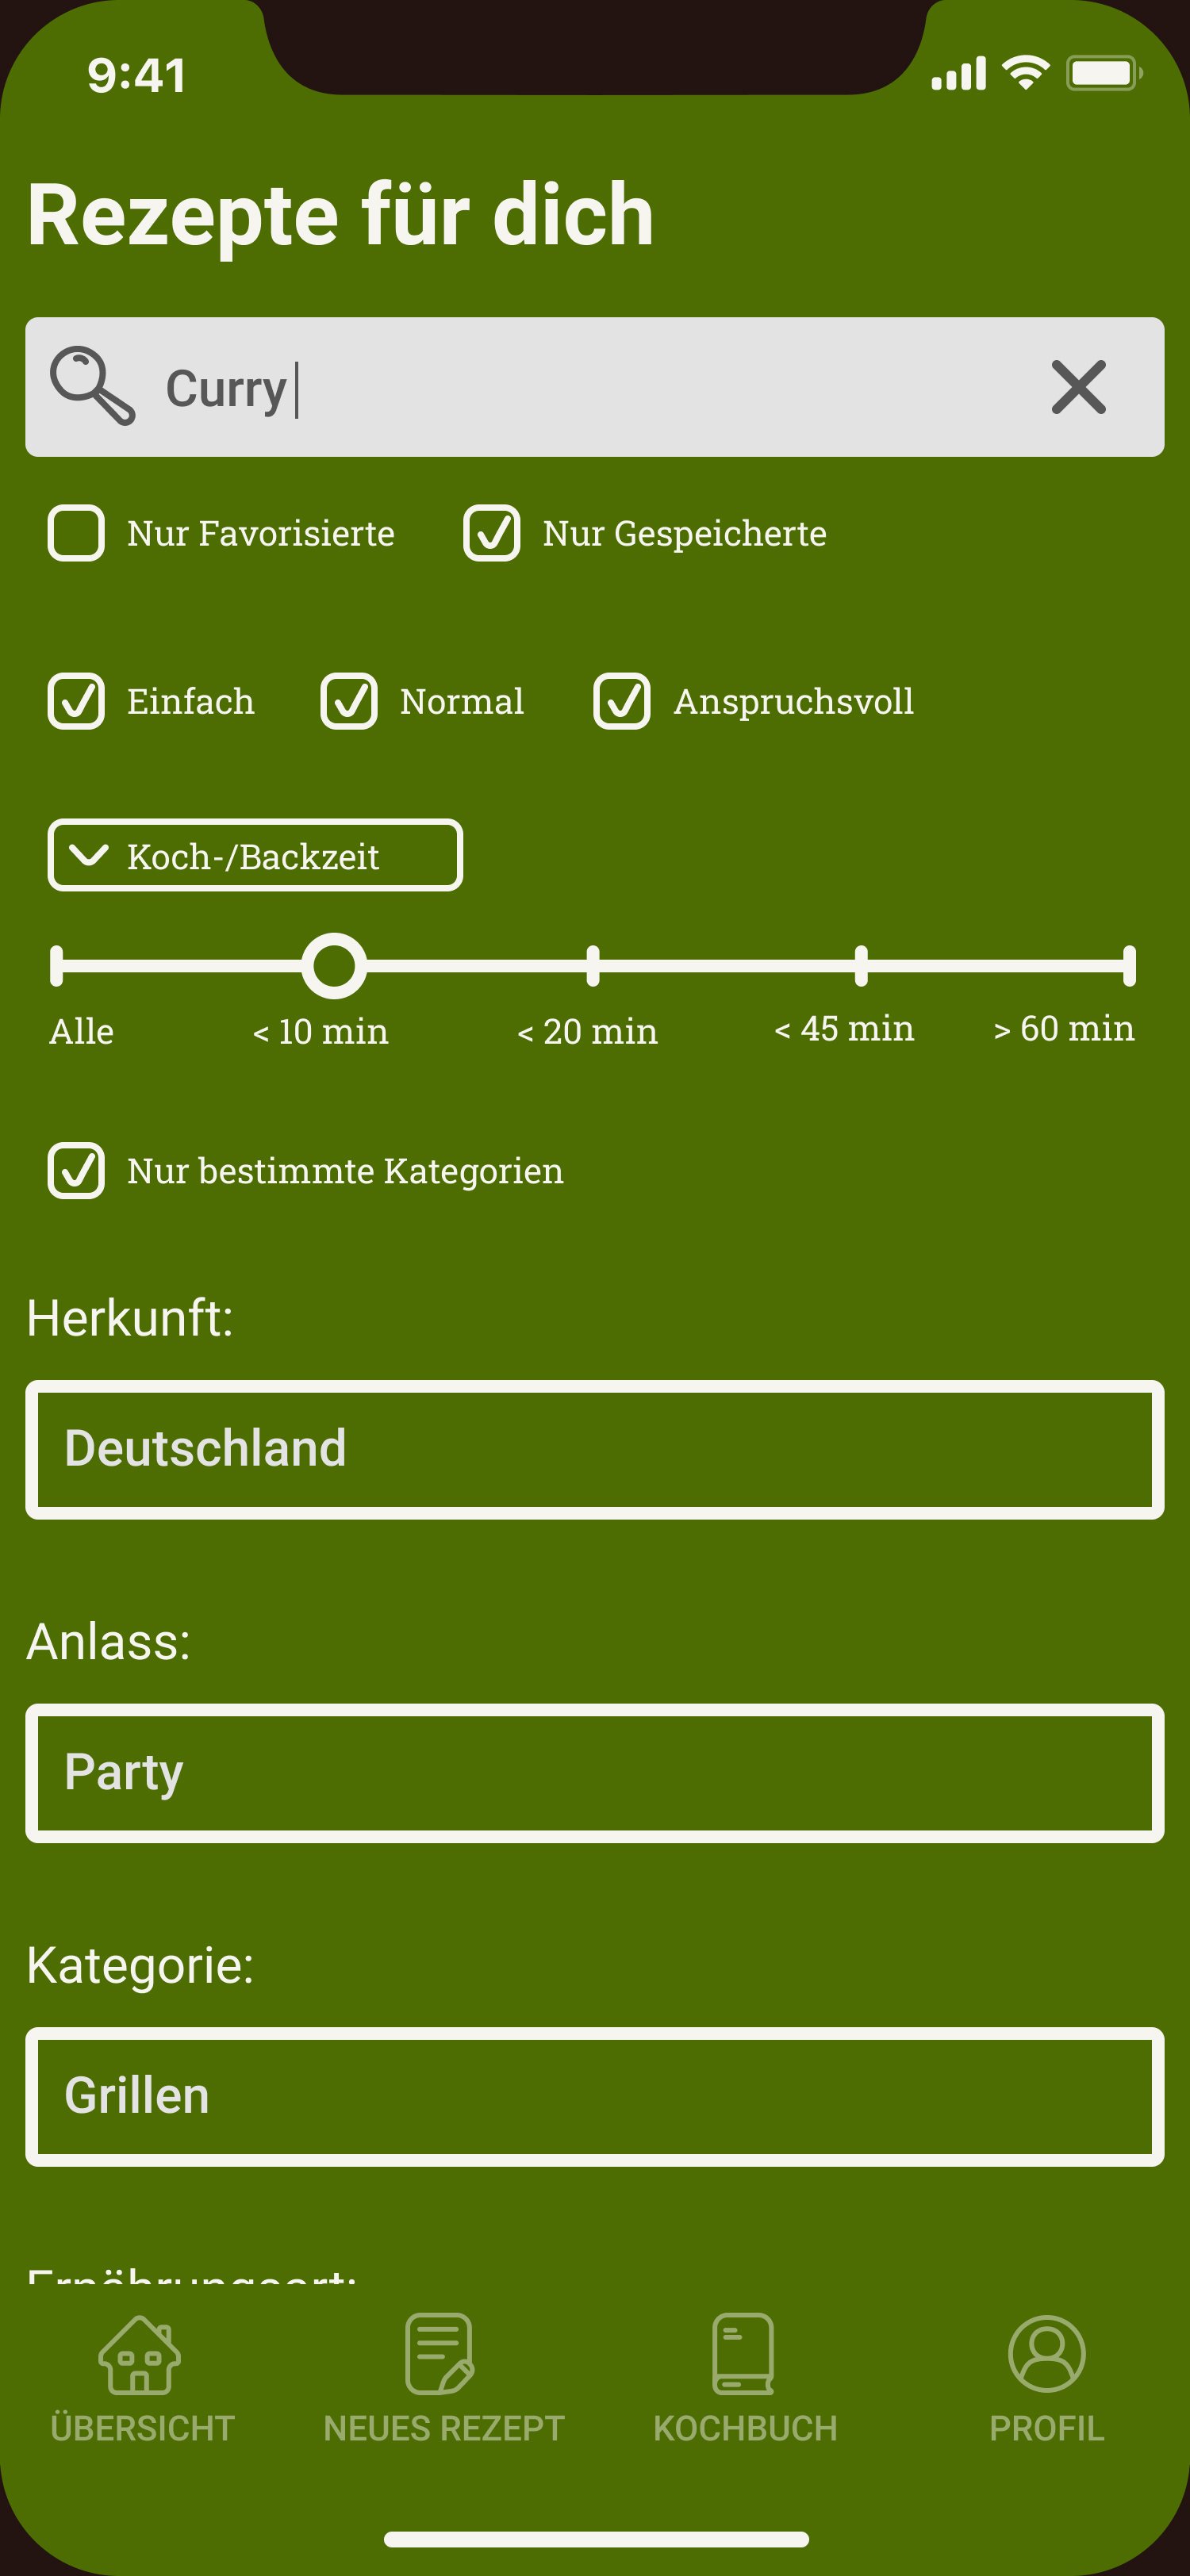
\includegraphics[width=0.14\textwidth]{images/filter.jpg}
    \caption[Mock Up - Filter]{Mock Up - Filter}
\label{fig:mockup-filter}
\end{wrapfigure}
Unter der Berücksichtigung der User Stories wurde entschieden, dass nach erfolgreichem Abschluss der Registrierung für den Dienst, im Sinne der Lernförderlichkeit, der Nutzer in das System eingeführt werden soll. Dabei werden die wichtigsten Funktionen mit interaktiven Beispielen visualisiert und mit Kommentaren erläutert. Der interaktive Prototyp umfasst die Einführung in das Finden von Freunden und Familienmitgliedern über die Kontaktsuche, das Hinzufügen von Kommentaren zu Rezepten, wichtige Teile des Anlegens eines Rezepts, die nachträgliche Rezeptbearbeitung, das Suchen und Filtern von Rezepten und das Teilen von Rezepten mit Kontakten. \\

Um die Suche nach Rezepten so intuitiv wie möglich zu gestalten, wurden anhand der User Stories Eigenschaften von Rezepten analysiert und diese dann, anhand von etablierten Interaktionsmustern, in interaktive Filter implementiert. Ein Beispiel dafür ist der Filter nach Zubereitungsdauer. Hier wurden die fünf durchschnittlich häufigsten Zubereitungsschritte gewählt und in einem verständlichen Slider implementiert. Auch Checkboxen, um bestimmte Eigenschaften eines Rezeptes in den Sucheregbnissen zu inkludieren oder zu ignorieren, sind Resultate dieser Analyse. Für Meta-Eigenschaften, wie die Herkunft eines Rezeptes, welche geringfügig mit der Zubereitung zu tun haben, wurde der Filter als Dropdown Menü, mit automatischer Vervollständigung, implementiert. Das soll die Nutzbarkeit erhöhen, aber auch wie der Filter selbst die Fehlertoleranz verbessern, da hier nur die Eigenschaftsdaten eingegeben werden können, welche auch tatsächlich in den für den Nutzer verfügbaren Rezepten vorkommt. \\

\begin{wrapfigure}{r}{0.38\textwidth}
    \centering
        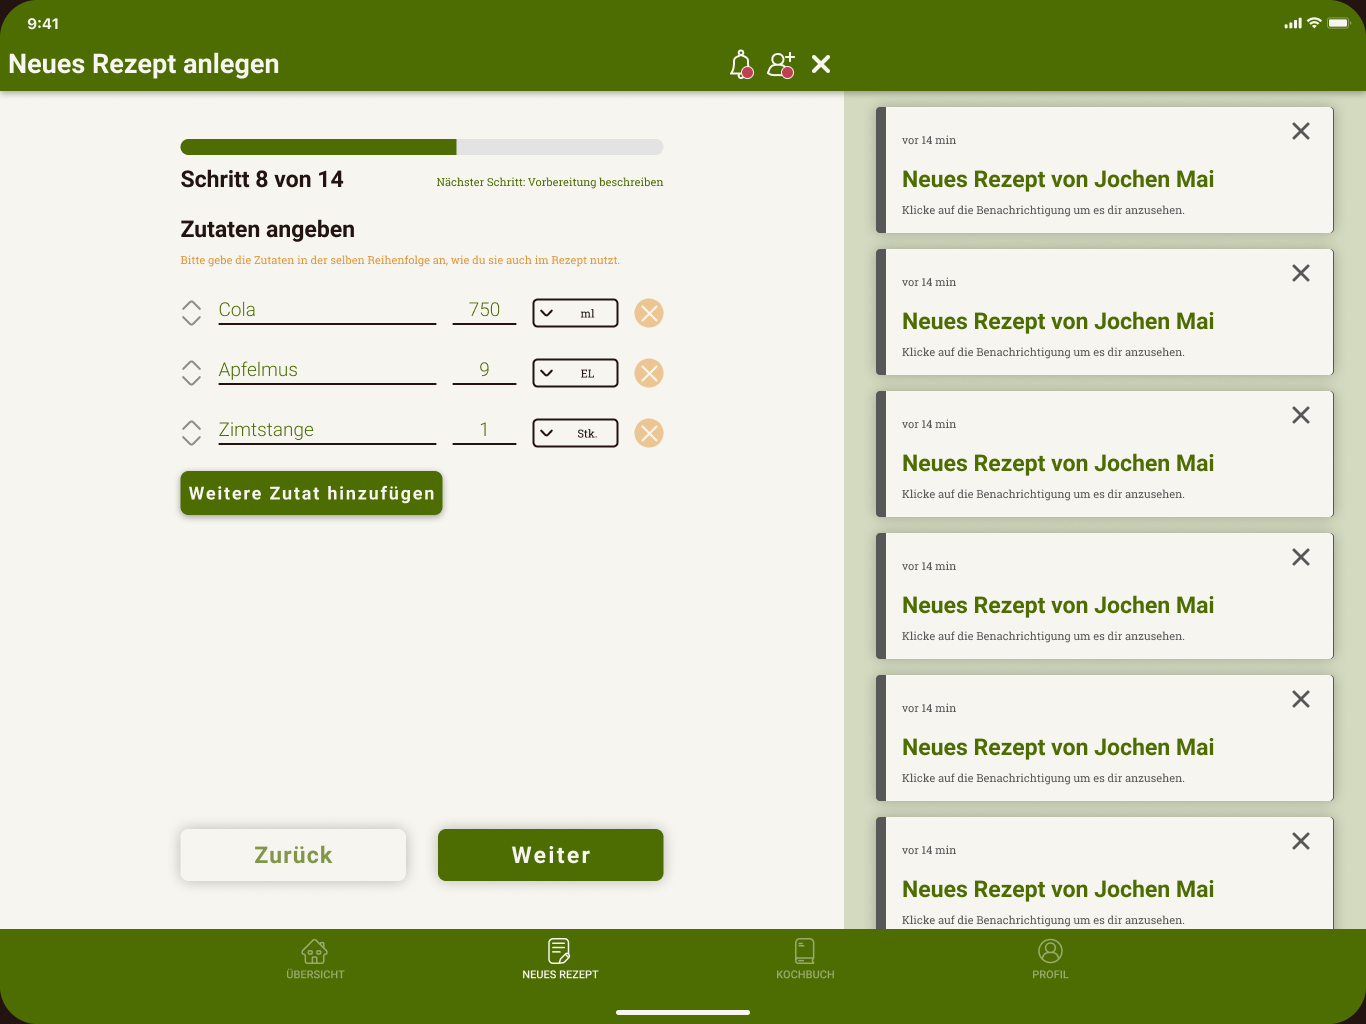
\includegraphics[width=0.38\textwidth]{images/addingredient.png}
    \caption[Mock Up - Zutaten angeben]{Mock Up - Zutaten angeben}
\label{fig:mockup-addingredient}
\end{wrapfigure}
Damit der Benutzer über Änderungen des Zustandes des interaktiven Systems informiert werden kann, wurde eine Fortschrittsanzeige implementiert, die sich am Kopf der Seite für das Anlegen eines Rezeptes befindet. Um den Bildschirm nicht zu überladen, wurden zusätzliche Informationen wie der Name des nächsten Schritts ausgeblendet. Für Desktop und Tablet Bildschirme sind diese Informationen jedoch verfügbar. \\

Im Sinne der Steuerbarkeit wurden die Buttons, ähnlich wie bei dem Blättern einer Seite in einem Buch, am unteren Bildschirmrand platziert und durch klare visuelle Unterschiede hierarchisiert. So ist der Button für das Fortsetzten der Bearbeitung mit der primären Farbe unterlegt und der Button für zurück farblich invertiert, was die invertierte Funktionalität wiedergibt. Der Button für das Überspringen eines Schrittes ist nur dann eingeblendet, wenn ein Schritt, für das Nachkochen, nur gering priorisiert wurde. Der Button wurde mit der Variante ausgewählt, die für die Nutzer die geringste Bedeutsamkeit hatte. \\

\begin{wrapfigure}{r}{0.38\textwidth}
    \centering
        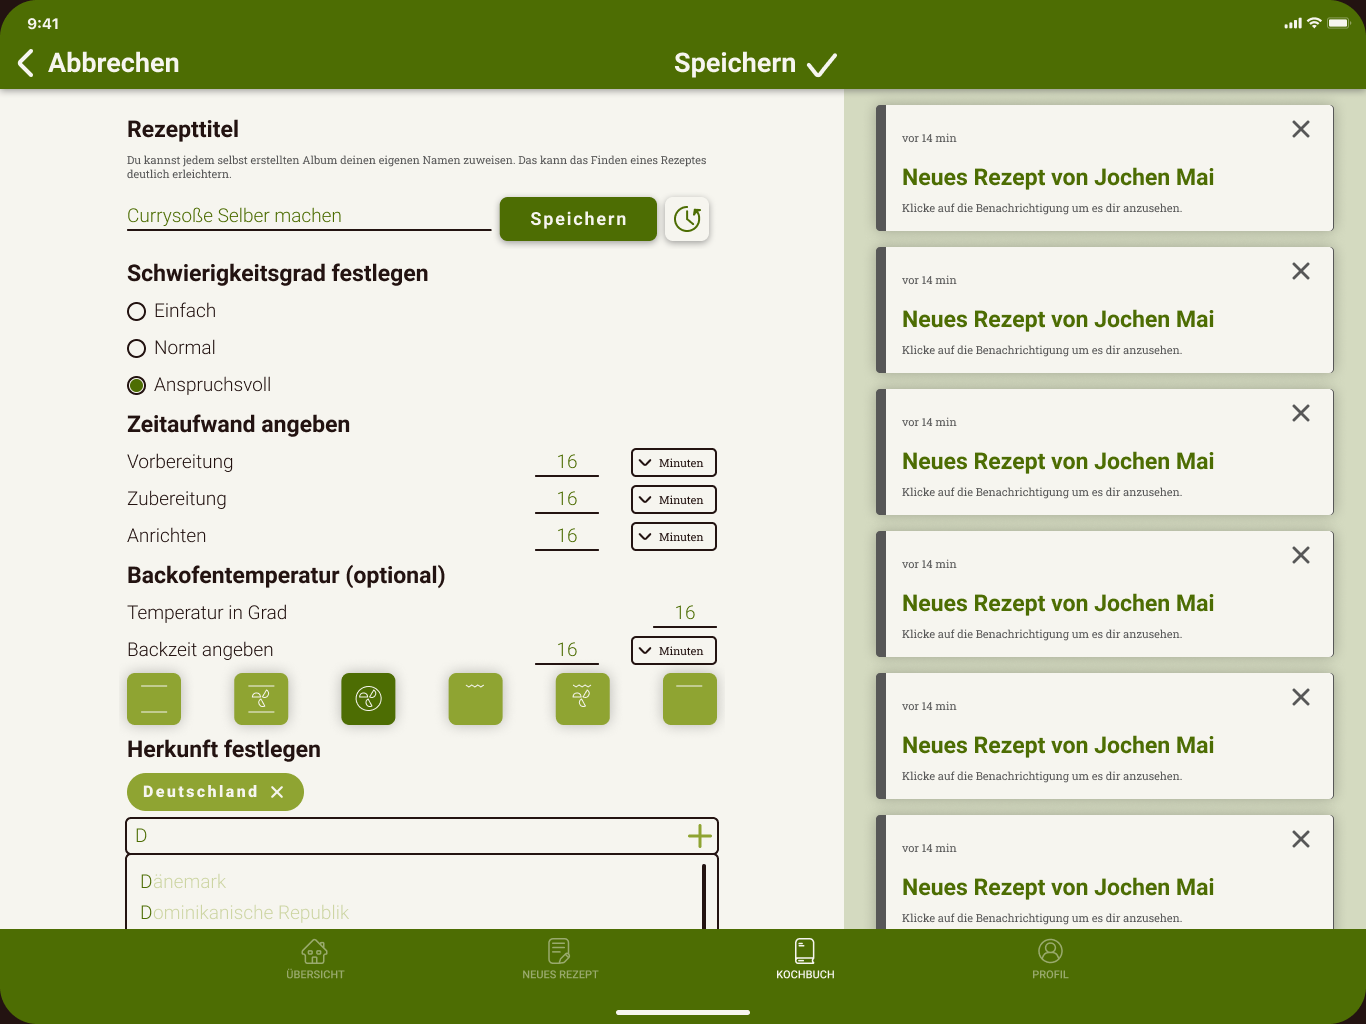
\includegraphics[width=0.38\textwidth]{images/editrecipe.png}
    \caption[Mock Up - Rezept bearbeiten]{Mock Up - Rezept bearbeiten}
\label{fig:mockup-editrecipe}
    \centering
        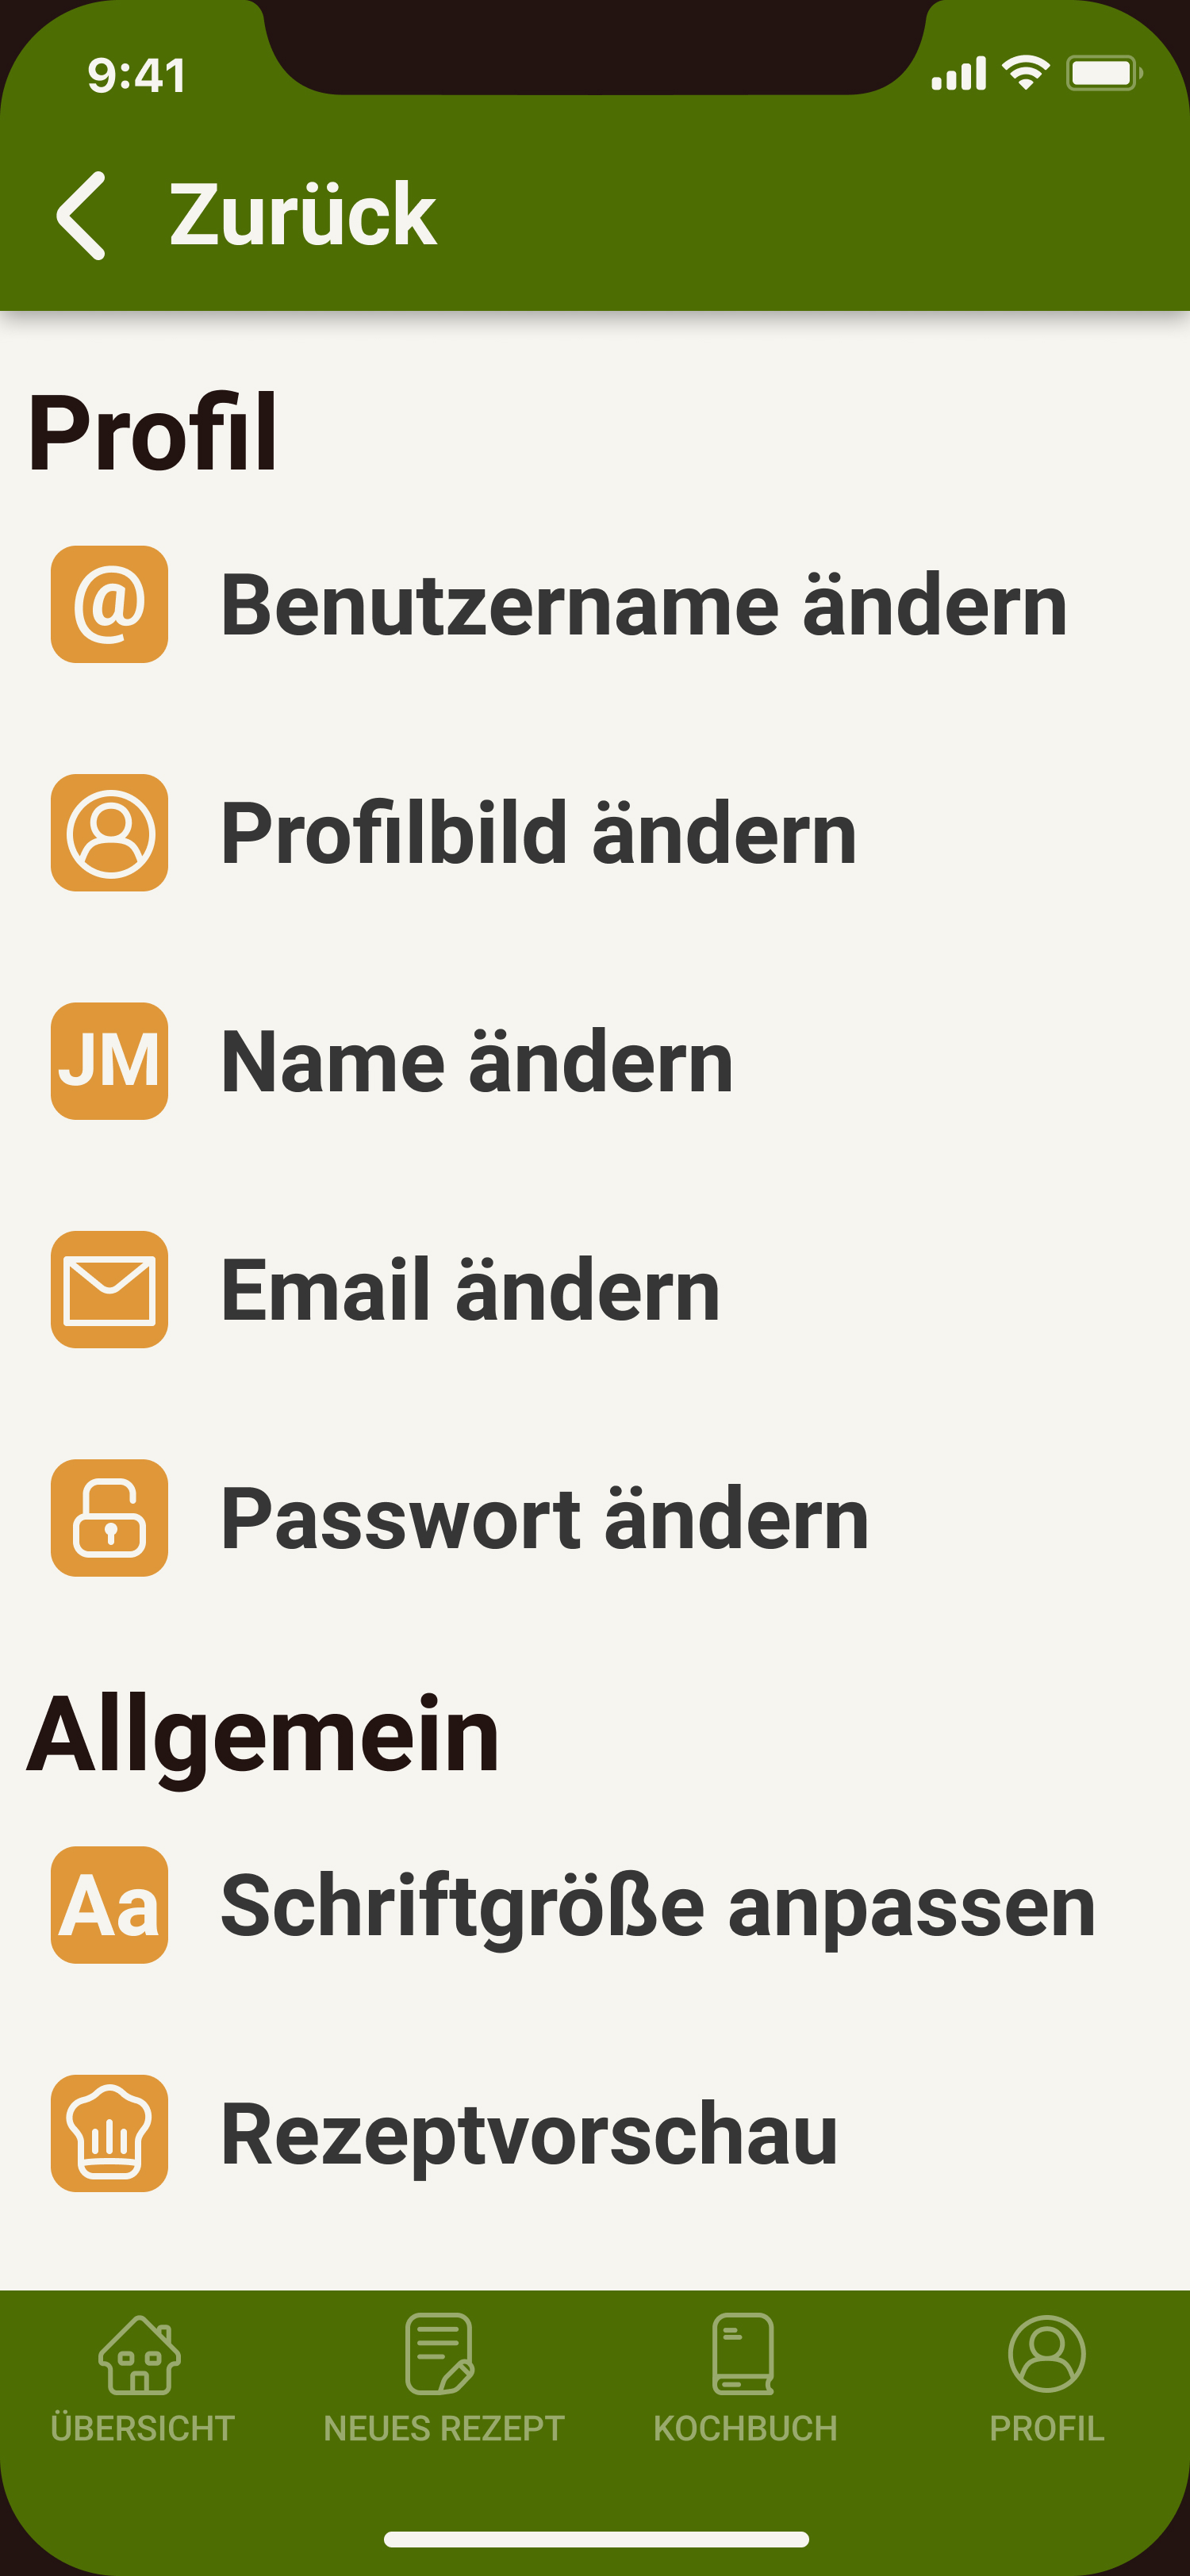
\includegraphics[width=0.14\textwidth]{images/settings.jpg}
    \caption[Mock Up - Einstellungen]{Mock Up - Einstellungen}
\label{fig:mockup-settings}
\end{wrapfigure}
Für das Mock Up aus Abbildung \ref{fig:mockup-editrecipe} wurde entschieden, dass wenn Nutzer ein Rezept bearbeiten wollen, sie das gesamte Rezept editieren müssen. In der späteren technischen Umsetzung soll es die Möglichkeit geben, an eine gewisse Stelle in der Rezeptbearbeitung zu springen, um ein ähnliches Verhalten, wie das Editieren einzelner Teile herzustellen. Für die Ergonomie sind die bereits bekannten Eingabevarianten der Rezepterstellung verantwortlich und die nutzerfreundlich platzierten Dialogsteuerungen in der Titelleiste für das Abbrechen oder Speichern der bisher getätigten Änderungen an dem Rezept. \\

Ein intuitiver Einstellungsscreen, der die Einstellungen eines Smartphones imitiert, bietet nicht nur die Konfigurationsmöglichkeit für Benachrichtigungen, Profil und Datenschutz, sondern auch für Schriftgröße und Akzentfarben des eigenen Kochbuchs und des gesamten Systems. Um das System nicht unbrauchbar durch Nutzeranpassungen werden zu lassen, sind die Auswahlmöglichkeiten dennoch auf ergonomische Alternativen beschränkt, mit Ausnahme der Akzentfarbe, welche über Hexadezimal-Codes oder einen Color-Picker verändert werden können. Diese Anpassungen sind der Individualiserbarkeit verschrieben. \\
\\
\\
% Lernförderlichkeit, Steuerbarkeit, (Fehlertoleranz), Individualisierbarkeit
% die anfänglichen Gestaltungslösungen befriedigen selten sämtliche Erfordernisse der Benutzer;
% Analysieren der Ergebnisse, Festlegen von Schwerpunktthemen und Unterbreiten von Lösungsvorschlägen;
\section{Prototypen}
Die Erarbeitung der Prototypen verlief nach dem \href{https://de.ryte.com/wiki/Mobile_First#Das_Prinzip}{Mobile First} \citep{mobilefirst:online} Prinzip. Dabei wird zuerst das mobile Design erarbeitet, um mögliche Probleme bei geringem Bildschirmplatz vorzubeugen. Beobachtet wurde jedoch der gegenteilige Effekt, da der bereits abgenommene Mobile Prototyp überarbeitet werden musste, nachdem es zu Problemen bei der Tablet Variante kam. \\ 

Das Designkonzept der Übersichts-Karten wurde komplett überarbeitet und ihnen mehr Platz eingeräumt, aber dafür auch mehr Weißraum \citep[vgl. Abschnitt {``Das Prinzip''}]{hegdewhitespace:online} innerhalb der Karten gegeben, was wiederum für ein nutzerfreundliches und aufgeräumtes Interface sorgen soll. Grund für die Änderung war das gedrückte Wirken der zuvor kleineren Karten und der mangelhaften Responsitivität. \\

Insgesamt wurden die Prototypen für alle in den User Stories enthaltenen Screens erarbeitet. Sie umfassen die Endgeräte Mobile (Iphone X), Tablet (Ipad Pro) und Desktop (MacBook Pro). Dabei handelt es sich nur um die Bildschirmgrößen. Zusätzlich wurden native UI Elemente der oben genannten Endgeräte eingebaut, um die Nutzung der Prototypen möglichst realistisch zu gestalten. \\

\begin{figure}[h] %!=overrides latex; h=here; t=top; b=bottom; p=special page for floating objects
    \center
    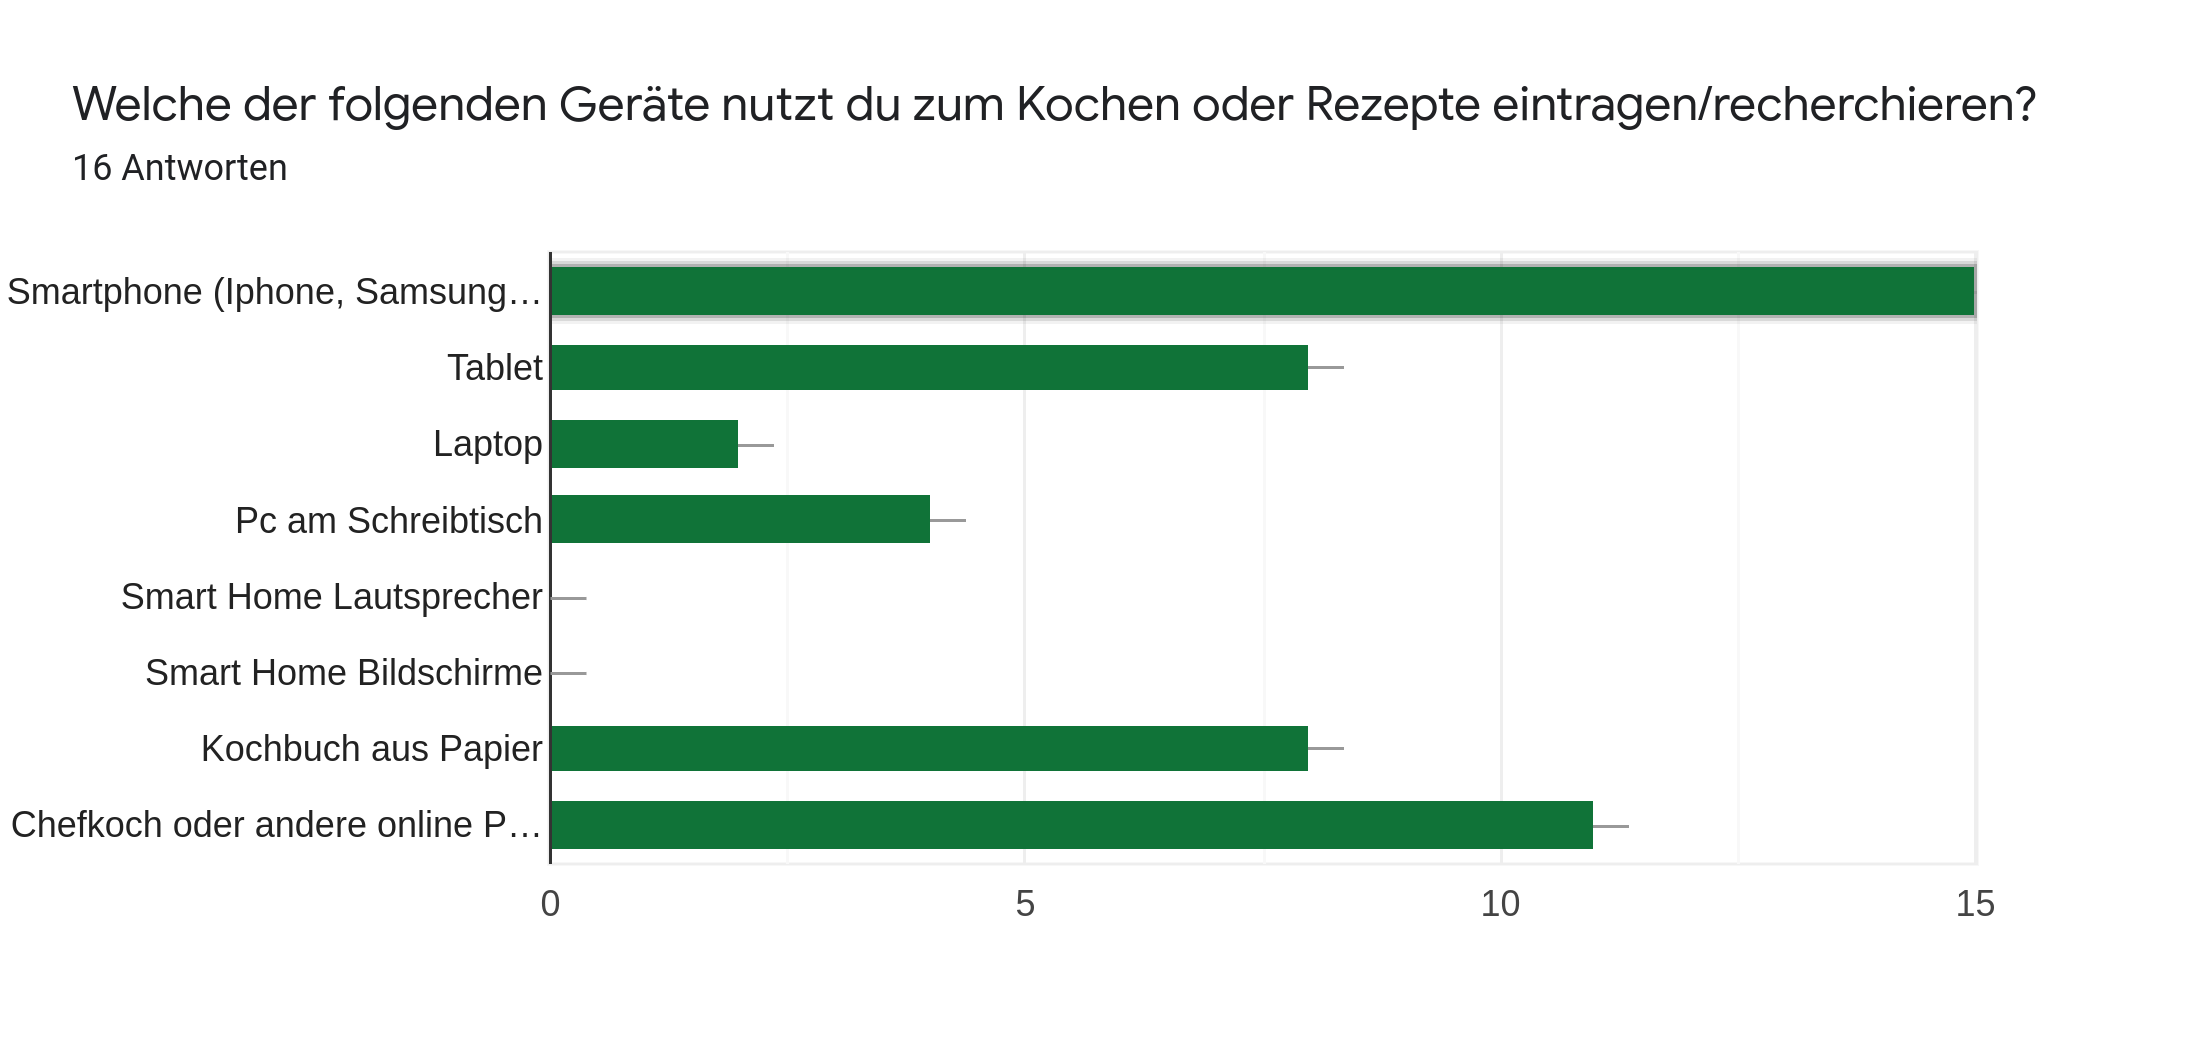
\includegraphics[width=0.8\textwidth]{images/recherchenutzung.png}
    \caption[Umfrage zur Nutzung der Geräte für die Recherche]{Recherche Nutzung Umfrage}
    \label{fig:recherchenutzung}
\end{figure}
Der Fokus des Systems liegt, bei dem Mobilen Prototypen, auf der Übersicht von Rezepten und Sozialen Interaktionen, wie Kommentare zu verfassen und Freunde zu verwalten, da anzunehmen ist, dass Nutzer ihr Smartphone tendenziell dafür nutzen, zu recherchieren (siehe \ref{fig:recherchenutzung}) oder sich mitzuteilen. \\

Für den Tablet Prototypen liegt der Fokus auf der Übersichtlichkeit der einzelnen Rezepte in der Detailansicht, um sie in der Küche leichter nachkochen zu können. Dabei können Rezepte im Portrait Modus angesehen werden. Das dient der verbesserten Übersichtlichkeit. \\ 

Für den Desktop Prototypen liegt der Fokus auf den Such- und Verwaltungsmethoden von Rezepten. So ist der Filter auf der rechten Sidebar sichtbar und die Suchergebnisse links in Karten-Form. Die Nutzer haben die Möglichkeit, alle wichtigen Filteroptionen zu jedem Zeitpunkt einzusehen und zu modifizieren. \\

Das Programm für die Erarbeitung und Evaluierung der Prototypen ist Figma, da es die Möglichkeit bietet, die Mock Ups um Interaktionen zu erweitern und dann auch interaktiv erfahrbar zu machen. \\

\begin{figure}[h] %!=overrides latex; h=here; t=top; b=bottom; p=special page for floating objects
    \center
    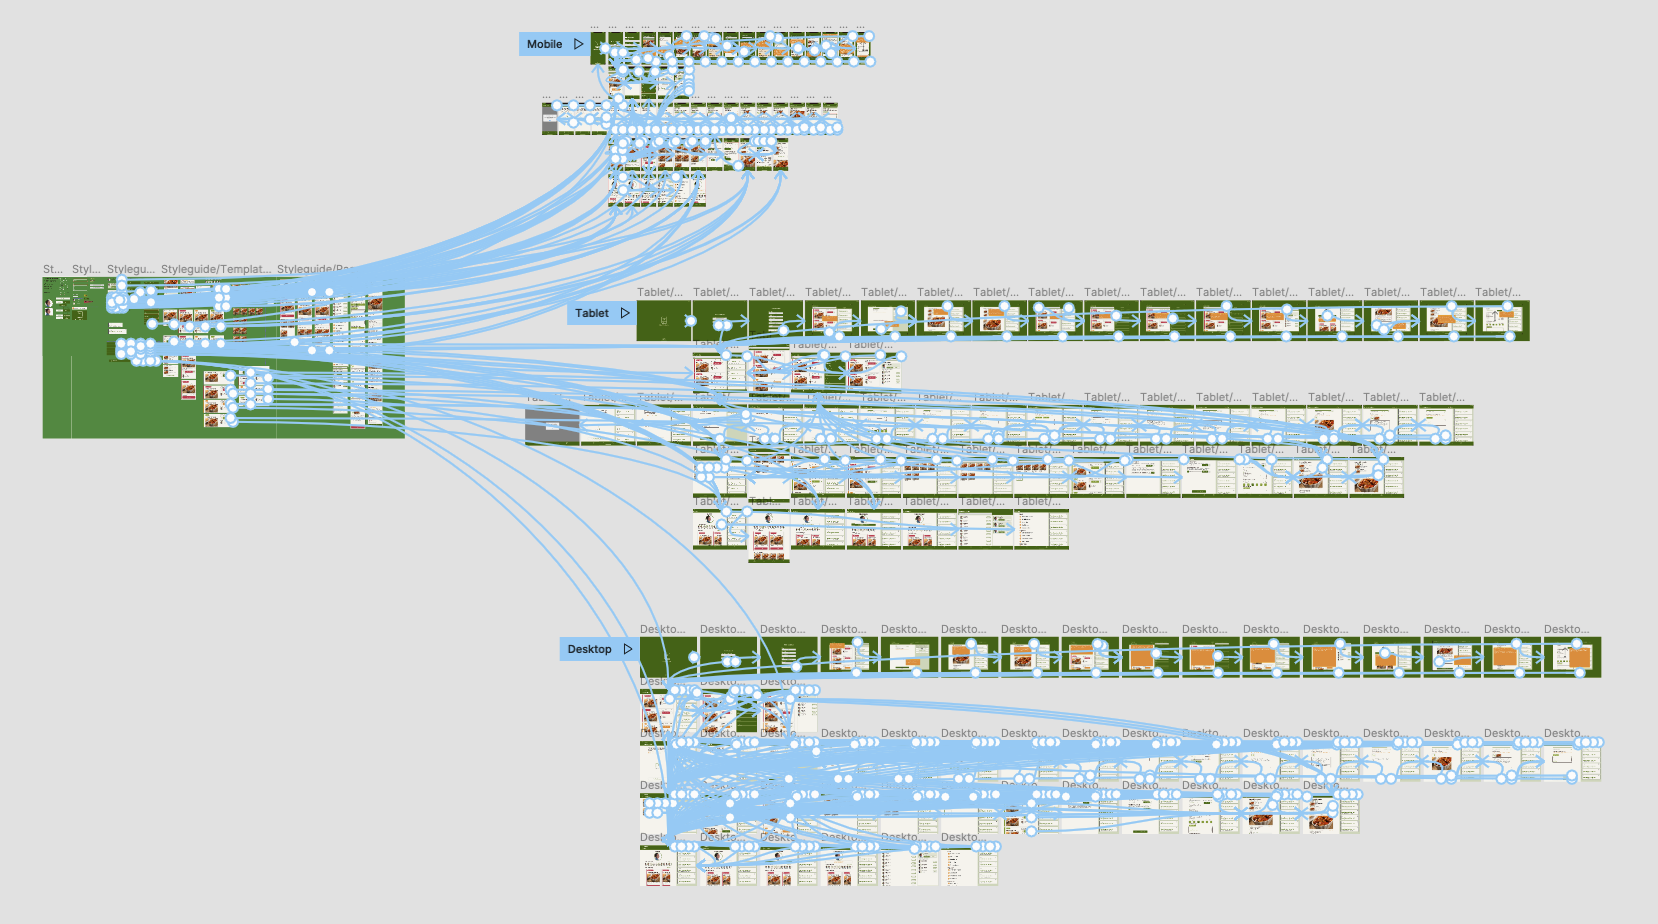
\includegraphics[width=0.8\textwidth]{images/prototyping.png}
    \caption[Prototypen in Figma]{Prototypen in Figma}
    \label{fig:prototyping}
\end{figure}

\section{Software Architektur}
Ausgehend von den User Stories aus \ref{sec:userstories}, lassen sich technische, aber Technologie unabhängige Anforderungen an das System ermitteln. 

\section{Minimum Viable Product (MVP)}
\begin{figure}[h] %!=overrides latex; h=here; t=top; b=bottom; p=special page for floating objects
    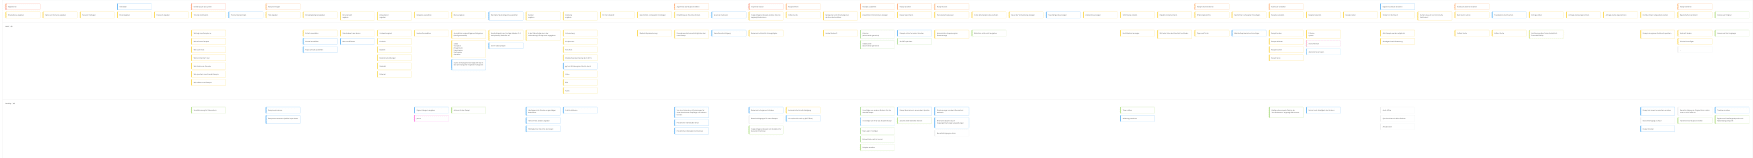
\includegraphics[width=1\textwidth]{images/mvp.png}
    \caption[Minimum Viable Product]{Minimum Viable Product}
    \label{fig:mvp}
\end{figure}
Während des Workshops wurden User Stories als zwingend notwendig bewertet und bildeten so das Rückgrat des MVPs. Mit fortlaufender Dauer des Workshops wurden Funktionen und Schritte an den verschiedenen Stellen ergänzt, was wiederum für ein langes, überfülltes Storyboard sorgte. Um diese User Stories in den MVP zu überführen, wurden die User Stories priorisiert und in {``Now''} und {``Not Now''} aufgeteilt.\\ 
Hier kam es zu längeren Diskussionen, da die Teilnehmer nicht immer einer Meinung waren. Das Ergebnis des Workshops bildet jedoch einen von allen Teilnehmern akzeptierten Kompromiss ab. Im Nachgang an den Workshop wurden diese Erwartungen und Erfordernisse in Anforderungen an das System und dessen Architektur überführt.\\

\section{Abhängigkeiten der Anforderungen}
\begin{wrapfigure}{r}{0.38\textwidth}
    \centering
    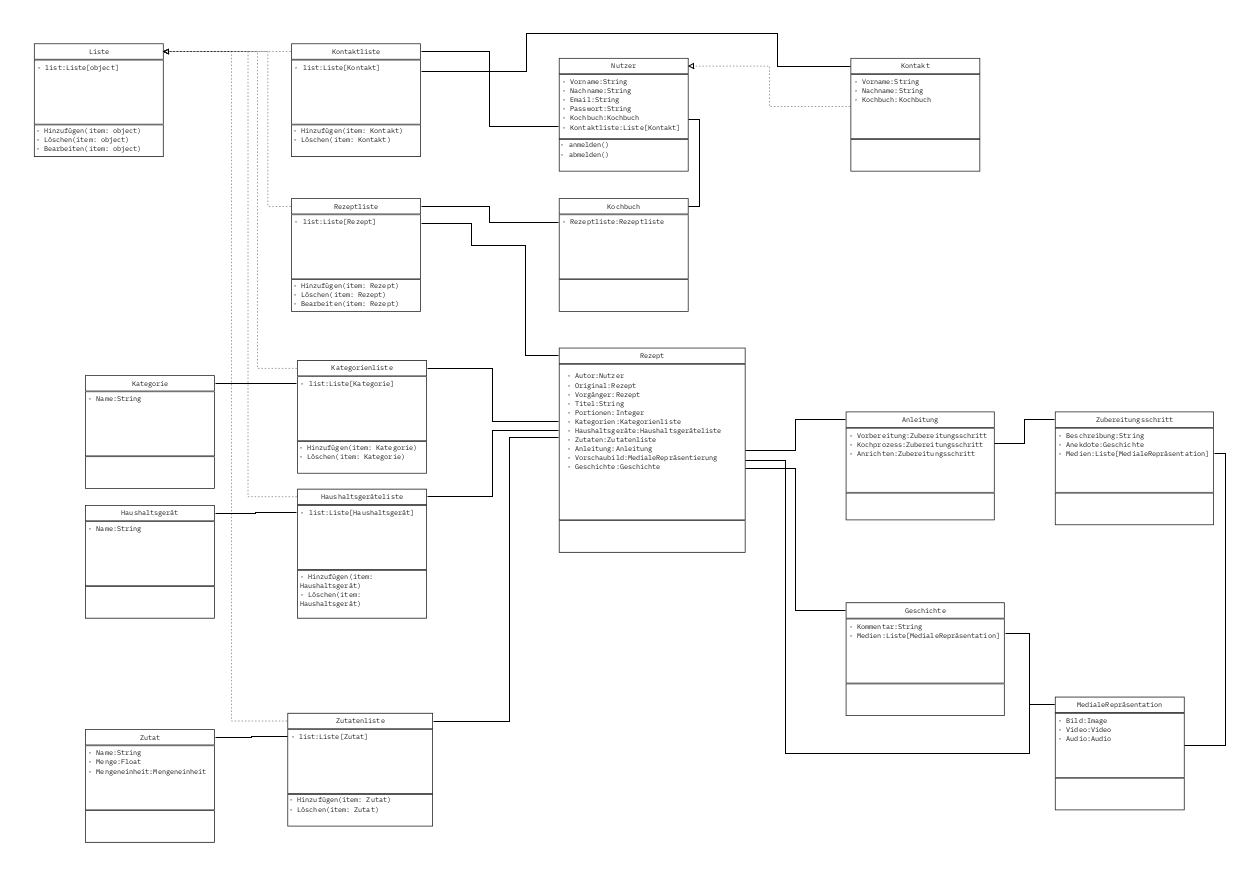
\includegraphics[width=0.35\textwidth]{images/dependencymodell.png}
    \caption[Abhängigkeitsmodell]{Abhängigkeitsmodell}
    \label{fig:dependencymodell}
\end{wrapfigure}
Die Anforderungen an das System wurden auf Abhängigkeiten untersucht und Lösungen für diese Abhängigkeiten oder daraus resultierende Folgen für das System notiert. In der Abbildung \ref{fig:dependencymodell} sind die Abhängigkeiten zwischen den zu speichernden Daten visualisiert. Um die gesammelten Lösungsansätze für die Abhängigkeiten weiter einzugrenzen, wurden konzeptionelle Lösungen, in einer Umfrage, den Nutzern präsentiert. Das Ergebnis der Umfrage hat die System Architektur maßgeblich geprägt.\\
\\

\section{Systemarchitektur}
\begin{figure}[h] %!=overrides latex; h=here; t=top; b=bottom; p=special page for floating objects
    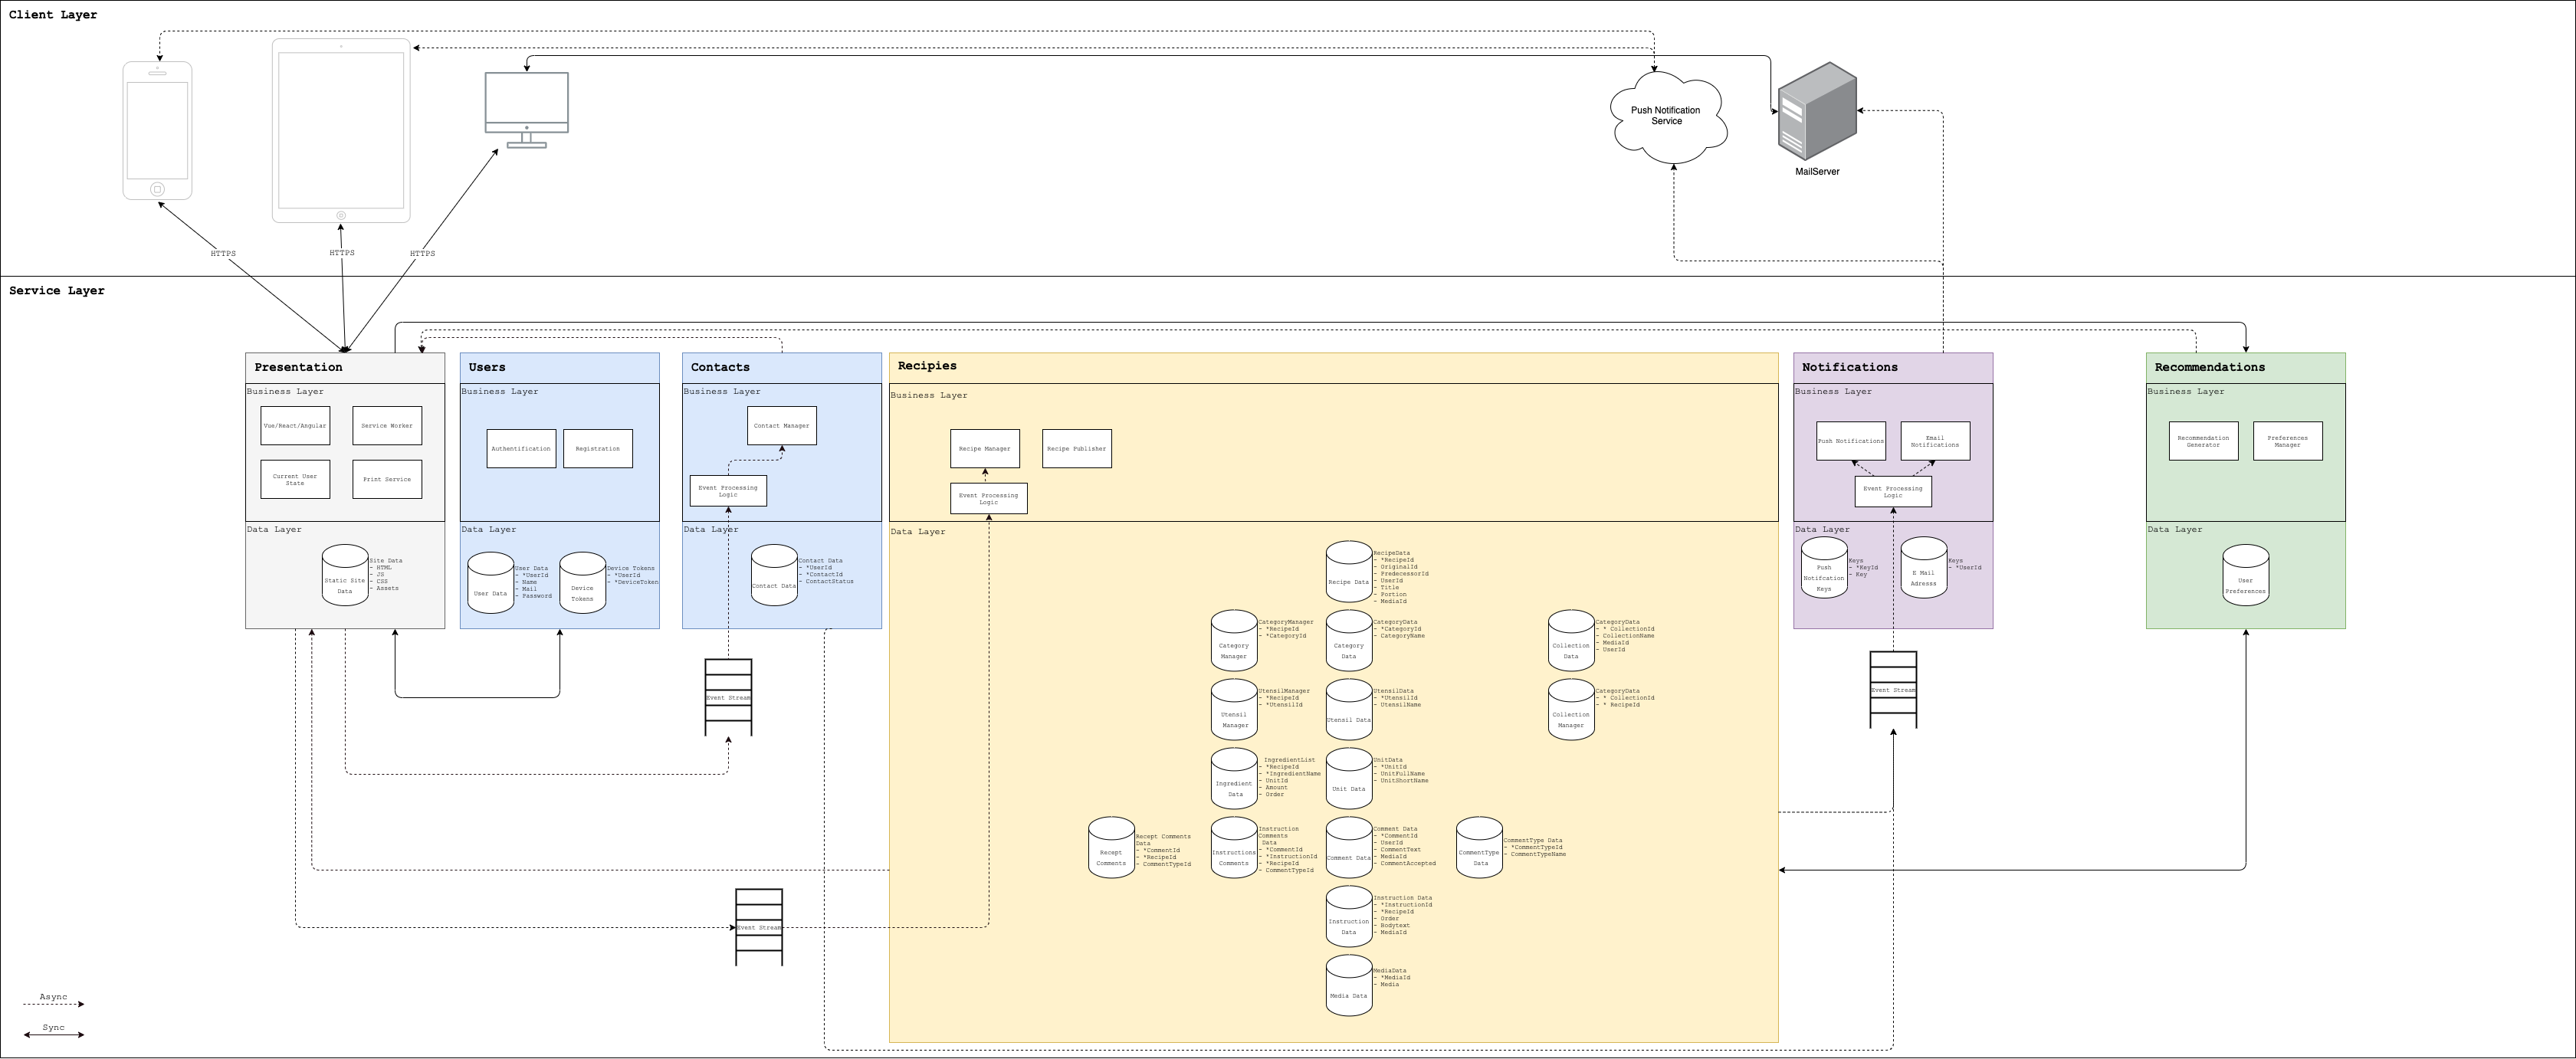
\includegraphics[width=1\textwidth]{images/systemarchitechure.png}
    \caption[Systemarchitektur]{Systemarchitektur}
    \label{fig:systemarchitechure}
\end{figure}
Das System wird auf zwei Ebenen liegen. Eine Ebene ist die Client Ebene. Hier wird die Anwendung auf den jeweiligen Endgeräten laufen und Benachrichtigungen empfangen. Die Service Ebene besteht aus 6 Service-Komponenten, welche jeweils eine bestimmte Aufgabe des Systems übernehmen. Diese Aufteilung soll das System skalierbarer machen und die Wartbarkeit fördern. Der Präsentationsservice stellt das Frontend über HTTPS den Endgeräten zur Verfügung und wird in JavaScript Frameworks, wie Vue oder React implementiert sein, da hier die Möglichkeit gegeben ist, aus einer Progressiven Web Applikation ohne großen Aufwand eine Native App zu generieren, was wiederum die Erreichbarkeit des Systems vergrößern würde.\\ 

Funktionen, wie die Druckfunktion, der Transfer von einem Rezept in HTML zu einem PDF zu exportieren und zu drucken oder die Funktionalität zu dem Lesen von Rezepten ohne aktive Internetverbindung, bieten den Nutzern zusätzliche Bequemlichkeit und Aufgabenangemessenheit. Die Servicekomponenten, für Clients und Kontakte, verwalten die Lese- und Schreibrechte für die Nutzer und sind daher essentiell für die Sicherheit des Systems.\\ 

Für die Rezepte ist ein relationales Datenbankschema angedacht, welches die Rezepte in einzelne Tabellen aufteilt, um den Abruf einzelner Informationen oder das Aktualisieren von Rezeptbestandteilen zu erleichtern. Das Modell und damit die Aufteilung der Komponenten, ist an die Content Map aus \ref{fig:navigationmap} angelehnt.\\ 

Die Benachrichtigungskomponente verfügt über den Anschluss an einen Mailserver des Systems und an Push Notfication Services, um Nutzer über neue Rezepte, nach Bedarf und individueller Einstellung, zu informieren. Die Empfehlungskomponente generiert in regelmäßigen Abständen Daten, die darüber Aufschluss geben sollen, welcher Nutzer welche Rezepte seines Bekanntenkreises mögen könnte, um so mit einer gewissen Wahrscheinlichkeit ihn dazu zu bringen, sich mit kulturell interessanten Rezepten zu beschäftigen. Zu beachten ist hier jedoch, dass noch keine Erfahrungswerte mit dieser Anwendungslogik bestehen und gewisse Parameter erst in der Alpha oder Beta Version des Systems optimiert werden können.\\

Die Komponenten sollen möglichst lose gekoppelt sein, bedürfen aber einiger Kommunikationsschnittstellen. Für die Kommunikation zwischen Client und Server ist eine REST Schnittstelle angedacht. Innerhalb des Systems jedoch wird auf asynchrone Kommunikation über Nachrichten gesetzt. Das System soll dadurch wartbarer, performanter und ausfallsicherer sein. \\

Zu bedenken ist jedoch, dass dieses Architekturmodell nur eine mögliche Lösung ist und sich gegebenenfalls während der Implementierung noch verändern könnte, aufgrund von der Änderung der Anforderungen oder der Nutzung effektiverer Technologien.
% einige Anforderungen zeigen sich erst dann, wenn ein Lösungsvorschlag vorliegt;
\section{Pseudocode}
\label{subsec:SimilarRecipes}
Für die Anwendungslogik der ähnlichen Rezepte unter einem angesehenen Rezept müssen zunächst Rezepte gekocht oder als gespeichert markiert worden sein. Als gekocht zählen Rezepte, welche über den Button als gekocht markiert wurden, oder länger als fünf Minuten betrachtet worden sind. Als gespeichert gelten die Rezepte, die über den Button als gespeichert markiert wurden. Die Dauer, die ein Nutzer ein Rezept betrachten muss, um es automatisch als gekocht zu markieren, ist noch nicht evaluiert und wird gegebenenfalls durch die Auswertung des MVPs angepasst. \\

Das aktuell betrachtete Rezept wird ausgewertet und dessen, als relevant betrachteten Attribute in dem Zwischenspeicher gesammelt. Für jedes markierte Rezept werden ebenfalls die relevanten Attribute gesammelt. Doppelt vorkommende Rezepte werden reduziert. Daraufhin werden alle markierten Rezepte durchlaufen und die Häufigkeit der vorkommenden Attribute inkrementiert. Daraus ergeben sich die Präferenzen des Nutzers einzelner Rezept-Bestandteile. Als Nächstes wird jedes Rezept, also gespeicherte, neue und unbekannte, durchlaufen. Für jedes Attribut, das im aktuell betrachteten Rezept  vorkommt, wird der Wert/Score des Rezepts erhöht. Für jedes Attribut das auch in den Präferenzen mit besonders hohem Vorkommen enthalten ist, wird der Score des Rezepts zusätzlich erhöht. Anschließend wird der Score des Rezepts durch die Anzahl seiner Attribute geteilt. Die Liste der Rezepte wird nach dem Score absteigend sortiert und dann die ersten fünf Ergebnisse zurückgegeben (siehe Pseudocode \ref{lst:SimilarRecipes}). Der Score ist ebenfalls ein Wert, welcher Feinjustierung benötigt.
\\ 
\label{subsec:Recommendations}
\\
Für die Empfehlung von Rezepten auf der Startseite sollen basierend auf der lokalen Zeit alle Menüs und Saisons gesammelt werden, um diese anschließend zusammen mit den Präferenzen des Nutzer, in einer Abfrage zu bündeln. Dabei werden alle verfügbaren Rezepten, die nicht das Menü oder nicht in der Saison enthalten sind, aus der Ergebnismenge entnommen. Anschließend werden Rezepte, die die Saison oder das Menü als Attribute enthalten, in ihrer Wichtigkeit erhöht. Das soll Rezepte, die weder ein Menü noch eine Saison gepflegt haben, in ihrer Wichtigkeit reduzieren, da sie bei der ersten Reduzierung der Ergebnismenge nicht entfernt wurden. Anschließend werden, wie zuvor beschrieben (siehe \ref{subsec:SimilarRecipes}), die persönlichen Präferenzen des Nutzers auf die übrig gebliebenen Rezepte angewendet und die fünf Rezepte zurückerhalten und ausgegeben (siehe Pseudocode \ref{lst:Recommendations}). \\

\chapter{Evaluierung der Gestaltungslösungen anhand der Anforderungen}
Für den letzten Schritt des Praxisprojekts, sollen die Gestaltungslösungen evaluiert werden und einen Zustand erreichen, bei dem die potenziellen Nutzer des Systems zufriedengestellt sind. \\

\section{Prüfung durch Benutzer}
% Qualitativ das Beste Ergebnis um die Frage zu beantworten
Im gesamten Projektverlauf wurden stets die einzelnen Artefakte von Benutzern evaluiert. Somit konnten die Teilnehmer wesentliche Bestandteile des interaktiven Systems durch ihre Kommentare beeinflussen. Die größte Beteiligung bestand bei der Auswahl der Schriftarten und textuellen Gestaltung eines gedruckten Rezepts. Hier sollten die Grundsteine für den zu entwickelnden Styleguide gelegt werden, um eine Richtung für die Mock Ups vorzugeben. Auch hier entstanden Meinungsverschiedenheiten zwischen den Nutzern, welche erst durch weitere Iterationen der Gestaltungslösung aufgehoben werden konnten. \\

\begin{figure}[h] %!=overrides latex; h=here; t=top; b=bottom; p=special page for floating objects
    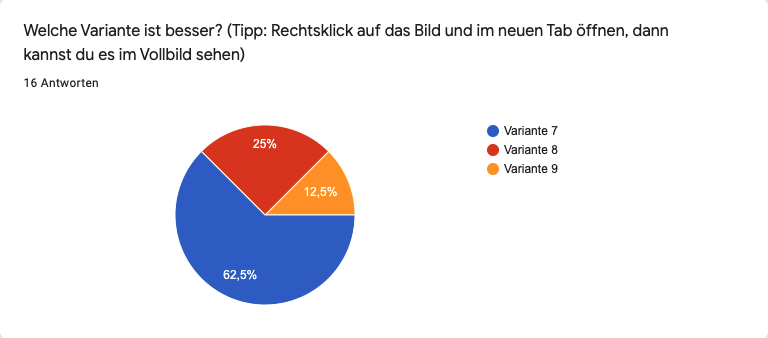
\includegraphics[width=1\textwidth]{images/EvaluierungBeispiel.png}
    \caption[Evaluierung - Beispiel]{Evaluierung - Beispiel}
    \label{fig:EvaluierungBeispiel}
\end{figure}

Im Nachgang an die durchgeführten Benutzerumfragen wurde nach dem höchsten Prozentsatz die Variante weiterentwickelt, bis eine Gestaltungslösung die größte Mehrheit erreicht hat. Während der Entwicklung der Mock Ups wurde eine wesentliche Anpassung der Karten, ebenfalls anhand von Benutzerumfragen, evaluiert und als die modernere, ergonomischere Lösung bewertet und folglich im gesamten Design umgesetzt. 

\section{Zeitliche Abstimmung und Ressourcen}
Im Rahmen des Praxisprojekts wurde die empirische Datenerhebung nur in kleinem Rahmen durchgeführt. Für die Bachelorarbeit sind Evaluierungen mit größeren Nutzergruppen angesetzt. Konkret bedeutet das, dass jeweils pro Umfrage fünf bis dreißig Personen interviewt worden sind oder an der Umfrage teilgenommen haben. Bedauerlich ist, dass die letzte Evaluierung deutlich weniger Beteiligung erfuhr aufgrund des ungünstigen Zeitpunkts um Weichnachten 2021 herum. Für kommende Projekte ist daher zu vermerken, dass in den Ferien im Sommer herum, die größte aktive Nutzerbeteiligung zu beobachten war.\\ 

Ebenfalls zu vermerken ist, dass das angeleitete Evaluieren eine bessere Methode darstellt, als die explorative Evaluierung, da nicht von jedem Nutzer zu erwarten ist, dass dieser seine Aufgabe gewissenhaft und gründlich löst. Eine User Story hingegen in eine Reihe von Aufgaben zu übersetzen und diese möglicherweise unter Beobachtung lösen zu lassen und die dabei erhaltenen Erkenntnisse zu dokumentieren, stellt die bessere Alternative dar. Mögliche Hilfestellungen bei der Findung von Ressourcen für die Evaluierung, stellen selbstverständlich Verteiler der Technischen Hochschule Köln, die Betreuer des Projekts, als auch Verbindungen durch den Arbeitgeber dar. Jedoch wurden diese aufgrund von zeitlicher Knappheit nicht in Anspruch genommen.\\ 
Die oben genannten Punkte sollen daher in der Evaluierung der Ergebnisse in kommenden Projekten, wie zum Beispiel der Bachelorarbeit beachtet und umgesetzt werden.

\chapter{Diskussion}
\label{cha:Diskussion}
% Zufrieden mit Feature Requests
\begin{figure}[h] %!=overrides latex; h=here; t=top; b=bottom; p=special page for floating objects
    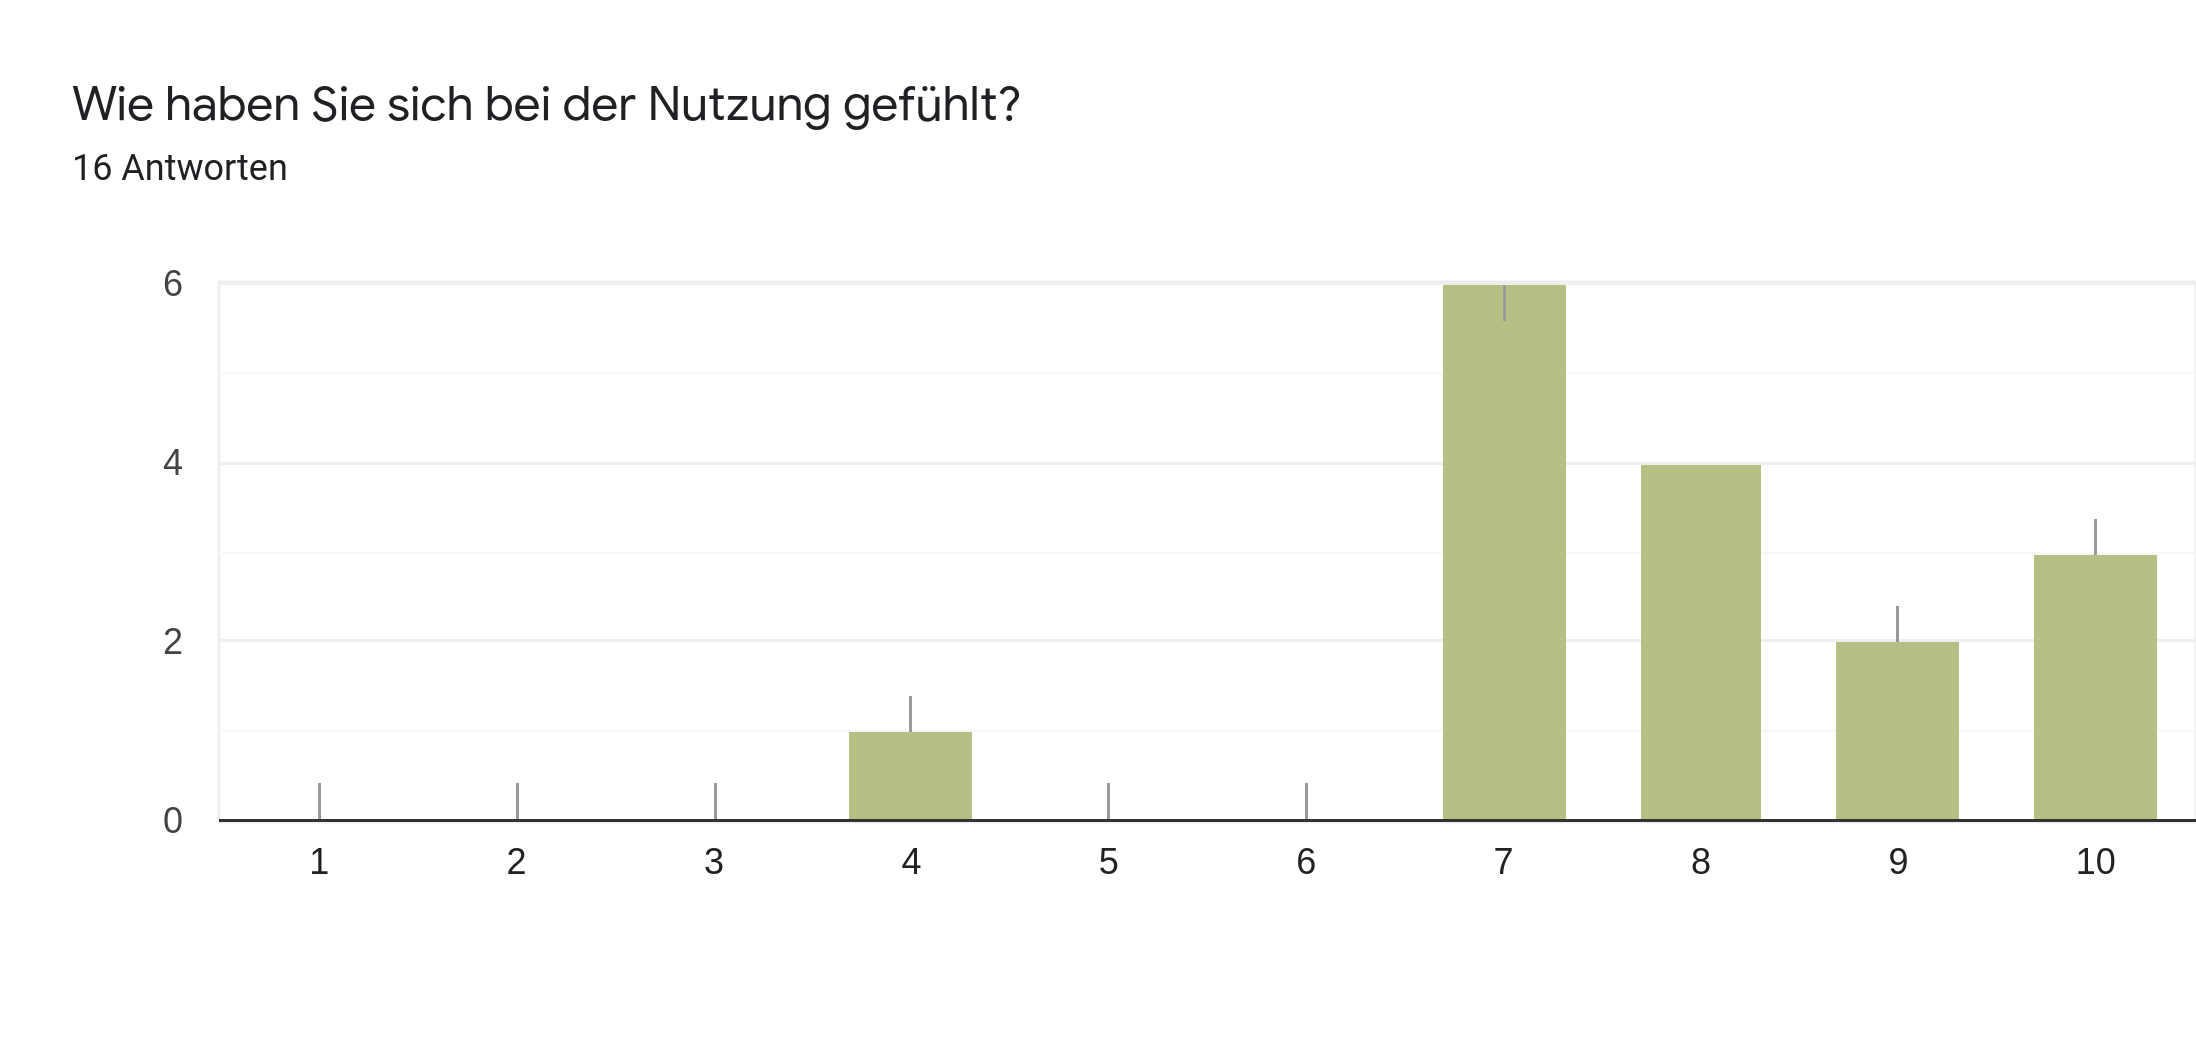
\includegraphics[width=1\textwidth]{images/PersonlichesEmpfinden.png}
    \caption[Evaluierung - Stimmungsbild]{Evaluierung - Stimmungsbild}
    \label{fig:EvaluierungStimmungsbild}
\end{figure}
An der abschließenden Befragung potenzieller Nutzer nahmen insgesamt 14 Personen teil. Dabei fielen die persönlichen Eindrücke der Nutzung größtenteils positiv aus. Ein Prozent gab an, eine subjektiv schlechte Erfahrung mit dem Prototypen gehabt zu haben. Ausgehend von den restlichen Bewertungen, scheint dies jedoch mit der Vertrautheit der älteren Personengruppen mit neuartigen digitalen Medien zu korrelieren.\\ 
Drei von insgesamt vier abgegebenen Bewertungen mit der Aussage {``Schwer''} stammen von über 45-jährigen Nutzern. 
Vier von insgesamt 14 abgegebenen Bewertungen mit der Aussage {``Einfach''} stammen von über 45-jährigen Nutzern. \\
Der Durchschnitt der Bewertung der Nutzererfahrung (1-10, weniger ist schlechter) liegt für über 45-jährige Nutzer bei 7.7 - für alle darunter, liegt der Durchschnitt bei 8. Anhand der abgegebenen persönlichen Kommentare lässt sich die schlechtere Bewertung so erklären, dass die Benamung einzelner Rezeptbestandteile irreführend empfunden wurde und es ihnen an Erklärungen für Interatkionsflächen mangelte.\\

42\% empfanden das Erstellen von Rezepten als einfach. Dagegen 14\% empfanden das angeleitete Erstellen eines Rezepts als schwer. Das Finden der eigenen Freunde und der privaten Rezepte bewerteten 57\% als einfach. 71\% gaben an, dass die Gestaltung der App ihren Erwartungen entspreche. Nur 41\%  gaben an, dass sie die Benutzung der App als ergnomisch oder intutiv bewerten würden. \\

Dies lässt darauf schließen, dass in kommenden Iterationen an den User Stories weiter entwickelt werden sollte oder mehr Nutzerüberflächen erklärt werden müssen. Ein weiteres Problem ist die Differenzierung von gespeicherten und favorisierten Rezepten. Diese Unterteilung wurde von 14\% Prozent nicht verstanden und kritisiert. Ein weiterer wichtiger Punkt ist die Kritik an der Schriftgröße. Diese wurden zwar nach den Guidelines und Fibunacci Skalen erstellt, der Evaluation ist  zu entnehmen, dass diese zu klein angesetzt sind und vergrößert werden müssen, um in der Praxis lesbarer zu sein.\\

Die Übersicht über die Vorgänger und Original Rezepte wurde als nicht wichtig bewertet und soll weiter unten an das Rezept angehangen werden, da es von dem eigentlichen Rezept ablenkt. Auch das Deaktivieren und Wechseln der Benachrichtigungsicons wurde kritisiert, da hier wohl die Bedeutung des Wechsels unklar ist. Im Gegensatz dazu wurde die Wahl der Icons als auch die Gestaltung von 42\% als positiv befunden. \\

Anhand des Stimmungsbildes aus der letzten Evaluierung (siehe \ref{fig:EvaluierungStimmungsbild}) lässt sich abschließend feststellen, dass die erarbeitete Gestaltungslösung, trotz reduzierter Funktionen und Individualisierungsmöglichkeiten sowie Fehler und Verbesserungsmöglichkeiten in der Erfahrung durch den Prototypen, bedingt durch die Limitierungen von Figma, die Nutzer zufriedenstellt.
Da Figma für die Darstellung des Prototypen, den Browser des jeweiligen Endgeräts benötigt, wurde ein Community Tool verwendet, um die Prototypen im Vollbildschirm auf dem Handy zu starten. Dadurch soll eine möglichst immersive Erfahrung geboten und die Evaluierung erleichtert werden. Das Tool trägt den Namen \href{https://figma.fun/}{Figma.fun} und wurde von Gleb Sabirzyanov entwickelt.\\

Manche Nutzer konnten nicht jede gestellte Aufgabe lösen und waren nicht in der Lage die interaktiven Teile des Prototypen auszumachen, obwohl in der Evaluierungsprotokoll-Einleitung als auch in der Einführung für die App, auf funktionale Dialogswege hingewiesen wurde. Als Lösung für dieses Problem soll ein Slider in der App implementiert werden, welcher Nutzer entscheiden lässt, wie viele Bedienungshilfen sie bei der Nutzung erhalten möchten. Dabei erhalten erfahrene Nutzer ein minimalistisches System mit selbsterklärenden Icons und geringerer Anzahl an Labels für Buttons. Unerfahrene Nutzer bekommen zusätzliche Hinweise. Wichtig ist, dass wichtige Hilfestellungen für eine positive Nutzererfahrung nicht reduziert werden sollen.\\
Mit der Implementierung des Sliders soll der identifizierte Mangel an Ergonomie zwischen den Altersklassen behoben werden.\\

% Im Diskussionsteil deiner Bachelorarbeit legst du deine Ergebnisse sowie die Folgen deiner Untersuchungen dar. Du evaluierst deine Ergebnisse und erläuterst, inwiefern sich Begrenzungen ergeben haben.
% Hier sprichst du ebenfalls Empfehlungen für weiterführende Forschung aus.
% Sind die Erkenntnisse erläutert und interpretiert worden?
% Sind Ursachen und deren Folgen klar dargestellt worden?
% Haben sich die Erwartungen erfüllt?
% Welche Hindernisse, Beschränkungen hat die Arbeit? Werden diese ausreichend dargelegt?
% Gibt es konkrete Anregungen für folgende Forschung?
% Ist der Aufbau der Diskussion logisch aufgebaut (anhand der Fragestellung, Hypothesen, chronologisch oder hierarchisch)?